% Elaborado para o X Workshop de Matematica e Matemática Aplicada
% (https://dmm.ufla.br/wmma/xwmma/).

\documentclass[12pt]{article}

% Linguagem
\usepackage[brazil]{babel}
\usepackage[utf8]{inputenc}

% Definir tamanho da página e margens
\setlength{\voffset}{-1,8cm}
\setlength{\hoffset}{-1,1cm}
\setlength{\textheight}{22,5cm}
\setlength{\textwidth}{16,0cm}


% Pacotes
\usepackage{amsmath}
\usepackage{makeidx}
\usepackage{graphicx}
\graphicspath{ {./images/} }
\usepackage[colorlinks=true, allcolors=blue]{hyperref}

\makeindex
\usepackage{amssymb}
\usepackage{theorem}
\usepackage{xcolor}
\usepackage[normalem]{ulem}
\graphicspath{{../figuras/}}
\usepackage{multicol}
\usepackage{wrapfig}
\usepackage{subfigure}
\usepackage{url}
\usepackage[multiple]{footmisc}
\usepackage{float}
\usepackage{pgfplotstable}
\usepackage{xfp}
\usepackage{siunitx}
\sisetup{
    locale=FR,
    round-mode=figures,
    round-precision=3,
    scientific-notation=true
}

\newtheorem{definicao}{Definição}
\newtheorem{Lema}{Lema}
\newtheorem{teo}{Teorema}
\newtheorem{prop}{Proposição}
\newtheorem{obs}{Observação}
\newtheorem{cor}{Corolário}
\newtheorem{ex}{Exemplo}
\newtheorem{exerc}{}
\newenvironment{dem}{\noindent{\bf Demonstração:} }{
\hfill $\Box$ \vspace{0.5cm}}


%%%%%%%%%%%%%%%%%%  SEU TEXTO %%%%%%%%%%%%%
%%%%%%%%%%%%%%%%%%%%%%%%%%%%%%%%%%%%%%%%%%%
\begin{document}
%\thispagestyle{empty}
\pagestyle{empty} %paginas sem numeracao
%\maketitle


\begin{flushleft}
\tiny {\textbf{X Workshop de Matemática e Matemática Aplicada
\hspace{5,0cm} Congonhas -- MG, 2025}}\\
\vspace{-0.175cm}
\hrulefill
\end{flushleft}

\begin{center}
    {\Large \bf Título}\\
\end{center}


% -----
\begin{flushright}
    {\footnotesize Bernardo Maia Coelho}\footnote{\label{nota1} Instituto de
    Ciências Matemáticas e de Computação -- Universidade de São Paulo, \\
    \texttt{fulano1@xxxxx.com.br}, \texttt{fulano2@xxxxx.com.br},
    \texttt{fulano3@xxxxx.com.br}} \\
    {\footnotesize Eduardo Fontoura Costa}
    \hyperref[nota1]{\textsuperscript{\ref{nota1}}} \\
    {\footnotesize Luiz Henrique Romero}
    \hyperref[nota1]{\textsuperscript{\ref{nota1}}}
\end{flushright}
\vspace{.6cm}

%%%%%%%%%%%%%%%%%%%%%%%%%%%%%%%%%%%%%%%%%%%%%%%%%%%%%%%%%%%%%%%%%%%%%%%%
% TEXTO
%%%%%%%%%%%%%%%%%%%%%%%%%%%%%%%%%%%%%%%%%%%%%%%%%%%%%%%%%%%%%%%%%%%%%%%%
\section{Formulação do Problema}

Dada uma função $f:\mathbb{R}^n \to \mathbb{R}^m$, buscamos uma aproximação por
combinação linear de funções base
$\Phi = \{\varphi_1,\varphi_2,\ldots,\varphi_k\} \subset V$, onde $V$ é o
espaço vetorial das funções $f$ dotado do produto interno
\begin{equation*}
    \langle f,g \rangle =
    \int_{\Omega}f(\vec{x})\cdot g(\vec{x}) \, d\vec{x},
\end{equation*}
com $\cdot$ denotando o produto escalar usual em $\mathbb{R}^m$ e
$\Omega \subset\mathbb{R}^n$ um domínio limitado e mensurável.
%
Para que esse produto interno esteja bem definido e seja finito, restringimos
nossa atenção às funções cujos componentes são quadrado-integráveis sobre o
domínio $\Omega$. Isso nos leva ao subespaço
\begin{equation*}
    V_\Omega = \{f\in V \mid f_i \in L^2(\Omega) \text{~para~} i=1,\ldots,m\},
\end{equation*}
o qual, quando dotado do produto interno acima, constitui um espaço de
Hilbert\cite{franco_calculo_numerico_2006}.

%
A linearidade do produto escalar em $\mathbb{R}^m$ permite reescrever o produto
interno entre $f,g\in V_\Omega$ como
\begin{equation*}
    \langle f,g \rangle =
    \int_{\Omega} \sum_{i=1}^{m} f_i(\vec{x}) g_i(\vec{x}) \, d\vec{x} =
    \sum_{i=1}^{m} \int_{\Omega} f_i(\vec{x}) g_i(\vec{x}) \, d\vec{x}.
\end{equation*}
Em particular, se adotarmos um domínio
$\Omega = [a_1,b_1]\times\ldots\times[a_n,b_n]\subset\mathbb{R}^n$, a
expressão acima assume a forma
\begin{equation*}
    \langle f(\vec{x}), g(\vec{x}) \rangle =
    \sum_{i=1}^{m} \int_{a_1}^{b_1} \cdots \int_{a_n}^{b_n}
    f_i(x_1, \ldots, x_n)
    g_i(x_1, \ldots, x_n) \, dx_n \cdots dx_1.
\end{equation*}
Quando a função $f$ é conhecida apenas por meio de uma amostragem em um conjunto
de pontos $\{p_j\}_{j=1}^N\subset\Omega$, é possível aproximar o produto
interno pela soma discreta
\begin{equation*}
    \langle f,g \rangle \approx
    \sum_{i=1}^m\sum_{j=1}^{N} f_i(\vec{p}_j)g_i(\vec{p}_j).
\end{equation*}
Com isso, o problema pode ser formulado como a resolução de um sistema linear
\begin{equation*}
    G\vec{a} = \vec{b},
\end{equation*}
conhecido como sistema de equações normais dos mínimos
quadrados\cite{burden_faires_2011,franco_calculo_numerico_2006},
em que $G\in\mathbb{R}^{k \times k}$ é a matriz de Gram, com entradas
$G_{i,j} = \langle \varphi_i,\varphi_j\rangle$; $\vec{a}\in\mathbb{R}^k$
contém os coeficientes da combinação linear; e $\vec{b}\in\mathbb{R}^k$ possui
entradas $b_i = \langle f,\varphi_i\rangle$.


\section{Regressão Polinomial}
\label{sec:regressao}

Uma forma natural e eficaz de construir uma base é por meio de polinômios,
sendo que o conjunto \(\{\varphi_k\}\) pode ser formado por todas as funções
da forma
\begin{equation*}
    \varphi_k = \hat{e}_d \, c_{d,\vec{\alpha}} \, x^{\vec{\alpha}},
\end{equation*}
onde o vetor de expoentes $\vec{\alpha} = (\alpha_1, \alpha_2, \ldots, \alpha_n)
\in \mathbb{N}^n$ varia sobre todas as combinações cuja soma é
$|\vec{\alpha}| = \sum_{i=1}^n \alpha_i \le r$ --- com $r$ sendo o grau máximo
do polinômio ---, e $\hat{e}_d \in \mathbb{R}^m$ é o vetor unitário com valor
$1$ na componente de índice $d$ e zero nas demais.
Portanto, o polinômio pode ser escrito como

\begin{equation*}
    P_{\le r}(\vec{x}) =
        \sum_{d=1}^{m}\;
        \sum_{\substack{\vec{\alpha}\in\mathbb{N}^n\\|\vec{\alpha}|\le r}}
        c_{d,\vec{\alpha}}\;\hat{e}_d\,\vec{x}^{\,\vec{\alpha}},
        \qquad
        \vec{x}^{\,\vec{\alpha}}:=
        \prod_{i=1}^{n} x_i^{\alpha_i}.
\end{equation*}

onde \(\vec{x}^{\,\vec{\alpha}}\) denota o monômio associado ao multi-índice
\(\vec{\alpha}\), conforme \cite{burden_faires_2011}.

Expandindo os termos homogêneos $x^{\vec\alpha}$, obtemos

\begin{equation*}
    P_{\le r}(\vec{x}) =
    \sum_{d=1}^{m} \;
    \sum_{j=0}^{r} \;
    \sum_{\substack{\vec{\alpha}\in\mathbb{N}^n\\|\vec{\alpha}|=j}}
    c_{d,\vec{\alpha}}\;\hat{e}_d\,
    \prod_{i=1}^{n} x_i^{\alpha_i}.
\end{equation*}

Note que aqui assumimos a existência de algum mapeamento razoável na forma

\begin{equation*}
    (d,\vec\alpha) \to k.
\end{equation*}

O índice $k$ referencia cada função base de maneira unívoca e nos permite adotar
a modelagem matricial usual: montamos o sistema linear $G\vec{a} = \vec{b}$ em
que $G$ é a matriz de Gram associada às $\{\varphi_k\}$.

\begin{equation*}
    \begin{bmatrix}
    \langle \varphi_0, \varphi_0 \rangle &
    \langle \varphi_0, \varphi_1 \rangle &
    \cdots &
    \langle \varphi_0, \varphi_n \rangle \\
    \langle \varphi_1, \varphi_0 \rangle &
    \langle \varphi_1, \varphi_1 \rangle &
    \cdots &
    \langle \varphi_1, \varphi_n \rangle \\
    \vdots & \vdots & \ddots & \vdots \\
    \langle \varphi_n, \varphi_0 \rangle &
    \langle \varphi_n, \varphi_1 \rangle &
    \cdots &
    \langle \varphi_n, \varphi_n \rangle \\
    \end{bmatrix}
    \begin{bmatrix}
        a_0 \\ a_1 \\ \vdots \\ a_n
    \end{bmatrix}
    = \begin{bmatrix}
        \langle f,\varphi_0 \rangle \\
        \langle f,\varphi_1 \rangle \\
        \vdots \\
        \langle f,\varphi_n \rangle
    \end{bmatrix}
\end{equation*}

Essa formulação estabelece as relações que serão usadas nas seções seguintes
para analisar o condicionamento numérico e as estratégias de solução.


\section{Otimização da Regressão}

Essa formulação já basta para viabilizar a modelagem computacional.
Ainda assim, convém enxergar onde estão os gargalos antes de escrever uma linha
de código.
O sistema linear proposto tem alta complexidade, e vale a pena organizar o
raciocínio desde já.
Seja $N_r$ o número de termos $\hat{e}_d\,\vec{x}^{\vec{\alpha}}$ de grau
igual a $r$ ($\|\vec{\alpha}\| = r$); então
\begin{equation*}
    N_j
    \; = \;
    m \cdot \#\{\vec{\alpha}\in\mathbb{N}^n:\ |\vec{\alpha}|=j\}
    \; = \;
    m\,\binom{n+j-1}{j}.
\end{equation*}

Assim, podemos calcular o número de termos existentes de grau até $r$
\begin{equation*}
    \| \{ \varphi_k \}\|
    \;=\;
    N_{\le r}
    \;=\;
    \sum_{j=0}^{r} N_j
    \;=\;
    m \sum_{j=0}^{r} \binom{n+j-1}{j}
    \;=\;
    m\,\binom{n+r}{r}.
\end{equation*}

Ou seja, a nossa matriz $G$ tem dimensão considerável:

\begin{equation*}
    N_{\le r} \times N_{\le r}
    = \bigl(m\,\binom{n+r}{r}\bigr)^2
    = m^2 \binom{n+r}{r}^2
    = m^2 \binom{n+r}{n}^2
    = m^2\,\frac{(n+r)!^{\,2}}{(n!)^{2}(r!)^{2}}.
\end{equation*}

Isso nos dá a complexidade para a regressão polinomial:

\[
    p=\binom{n+r}{r}.
\]

Via método QR:
\[
    T_{\mathrm{QR}}(N,n,r,m)=O\!\left(Np^{2}+p^{2}m\right)
\]

Via equações normais (Cholesky):
\[
    T_{\mathrm{NE}}(N,n,r,m)=O\!\left(Np^{2}+p^{3}+p^{2}m\right)
\]

Essas estimativas refletem a comparação clássica entre decomposição QR e
equações normais/Cholesky na resolução de mínimos
quadrados\cite{burden_faires_2011,franco_calculo_numerico_2006}.

Os fatoriais elevados a 2 ou 3 já são razão suficiente para deixar qualquer
cientista da computação em alerta.
Não conseguimos melhorar muito a complexidade assintótica desse algoritmo,
porém é possível extrair um ganho de desempenho prático explorando uma
propriedade estrutural de $G$.
Note que, por definição,
$$
\hat e_i \perp \hat e_j \quad i \ne j \quad \implies
\langle \hat e_i \; c_{d,\vec{\alpha}} \; \vec x ^{\vec \alpha},
\hat e_j \; c_{d,\vec{\beta}} \; \vec x^{\vec \beta}\rangle = 0
$$

Então, com uma boa escolha de mapeamento do índice $k$, nossa matriz $G$
torna-se diagonal por blocos:

$$
A \;=\;
\begin{array}{ccc}
  &

    e_1 \quad\;e_2 \quad\; \cdots \quad\; e_n

  & \\[1ex]
%
  \left. \,
    \begin{matrix}
      e_1\\
      e_2\\
      \vdots\\
      e_h
    \end{matrix}
  \right.
  &
    \begin{bmatrix}
      A_1      & 0        & \cdots & 0      \\
      0        & A_2      & \cdots & 0      \\
      \vdots   & \vdots   & \ddots & \vdots \\
      0        & 0        & \cdots & A_h
    \end{bmatrix}
  &
  \left.
    \begin{matrix}
      \\ \\ \\
    \end{matrix}
  \right.
\end{array},
$$

Usando o delta de Kronecker, podemos resumir essa propriedade da seguinte forma:

$$
    G_{ij} =
    \langle \varphi_i ,\, \varphi_j \rangle \cdot
    \delta_{i ,\, j}
    ,\quad\quad
    \hat e_i \perp \hat e_j
$$

Logo, em vez de resolver um sistema linear de tamanho catastrófico, exploramos
as propriedades de matrizes diagonais por bloco e decompomos o problema em $m$
sistemas menores do tipo
$$A_i \, a_i = b_i.$$

Essa estratégia não altera a complexidade assintótica, mas proporciona um ganho
de desempenho prático relevante.
Além disso, como as matrizes $A_i$ são idênticas entre si --- variando apenas o
vetor unitário associado a cada componente ---, é possível reutilizar
artefatos intermediários e paralelizar os solvers sem esforço adicional.



\section{Metodologia}
\label{sec:metodologia}

A metodologia seguiu diretamente a formulação dos mínimos quadrados apresentada
nas Seções iniciais. As bases polinomiais descritas em $\S$\ref{sec:regressao}
foram geradas tanto pela abordagem simbólica quanto pela implementação
vetorizada do pacote \texttt{regkit}, garantindo que os sistemas normais
$G\vec{a}=\vec{b}$ produzidos em cada experimento correspondessem à teoria. A
versão simbólica atuou como referência para depuração, enquanto a variante
otimizada foi empregada nas execuções de larga escala descritas a seguir.

\subsection{Problemas estudados}

Foram analisados três problemas complementares. O primeiro é o conjunto
exploratório de hélices gerado por \texttt{gen\_exploration\_dataset}, com
$n=3$, $m=2$, $N=200$ e ruído gaussiano de desvio padrão $0{,}01$. Ele codifica
trajetórias helicoidais acopladas entre entradas e saídas e serve como cenário
controlado para validar a montagem matricial e comparar as implementações
ingênua e vetorizada. O segundo problema corresponde ao protótipo~4$\times$4,
conjunto alvo sintético obtido por \texttt{create\_target\_dataset} que
reproduz a versão estruturada em MATLAB com quatro entradas e quatro saídas
parametrizadas pelos eixos temporais $t$ e $q$. A heterogeneidade entre os
regimes de tempo e parâmetro torna esse protótipo o foco principal da aplicação.
O problema extra é o ajuste da superfície ``wing'' a partir de 308 amostras
avaliadas sobre a geometria da asa. 

\subsection{Procedimentos experimentais e visualização}

Cada execução foi gerenciada pelos scripts \texttt{run\_regkit\_usage.py} e
\texttt{run\_benchmark\_regression.py}. O primeiro instancia os problemas das
hélices e do protótipo~4$\times$4, executa um \textit{sweep} nos graus polinomiais de
1 a~10 e persiste as métricas de erro em \texttt{results/regkit\_usage\_rmse.csv}.
O segundo consolida os experimentos da asa e os benchmarks de desempenho. A
análise qualitativa utiliza o utilitário \texttt{plot\_dataset}, que aplica PCA
em $\mathbb{R}^{n+m}$ e reaproveita o mesmo projetor para comparar dados
originais e predições. Esse procedimento mantém a
correspondência geométrica entre séries reais e estimadas, além de orientar a
leitura dos resíduos nas figuras apresentadas na Seção~\ref{sec:resultados}. 
Vale ressaltar que a utilização do PCA é necessária para visualizar a semelhança 
entre os conjuntos, dada a alta dimensionalidade dos dados. Apenas o problema da asa
permite uma visualização direta, pois ocorre em três dimensões. 

\section{Implementação}

\graphicspath{{img/}{../img/}{../../img/}}

\pgfplotstableread[col sep=comma]{../../results/optimized_largeP_metrics.csv}\streammetrics

\pgfplotstablegetelem{0}{rmse}\of\streammetrics
\edef\streamFullRmse{\pgfplotsretval}
\pgfplotstablegetelem{1}{rmse}\of\streammetrics
\edef\streamIncrementalRmse{\pgfplotsretval}
\pgfplotstablegetelem{0}{coef_diff_fro}\of\streammetrics
\edef\streamFullCoefDiff{\pgfplotsretval}
\pgfplotstablegetelem{1}{coef_diff_fro}\of\streammetrics
\edef\streamIncrementalCoefDiff{\pgfplotsretval}

Os protótipos desenvolvidos ao longo da pesquisa foram consolidados no pacote
\texttt{regkit}, estruturado para atender a duas demandas complementares. A
primeira trata da reprodução fiel da formulação simbólica discutida nas seções
anteriores. Para isso, o módulo \texttt{naive} emprega a biblioteca SymPy para
gerar automaticamente todos os monômios até um grau $r$ e combina cada termo
com os versores $\hat e_d$ associados às saídas. Em seguida, as funções
lambdificadas são avaliadas ponto a ponto para montar a matriz de Gram $G$ e o
vetor $b$ do sistema normal $G\vec{a}=\vec{b}$, preservando a estrutura em
blocos descrita anteriormente.

\begin{equation*}
    G_{ij} =
    \sum_{p=1}^{N} \varphi_i(\vec{x}_p) \cdot \varphi_j(\vec{x}_p),
    \qquad
    b_i = \sum_{p=1}^{N} f(\vec{x}_p) \cdot \varphi_i(\vec{x}_p).
\end{equation*}

Embora computacionalmente onerosa, essa rota permitiu validar cada etapa da
derivação original e gerar códigos numéricos equivalentes via SymPy, que
serviram como referência para os demais experimentos.

A segunda demanda é a execução eficiente em cenários com muitos pontos
amostrais. O módulo \texttt{optimized} codifica diretamente a montagem por
blocos, utilizando a transformação \textit{PolynomialFeatures} do
\textit{scikit-learn} para obter a matriz de projeto $V \in \mathbb{R}^{N \times
Q}$. Dessa forma, o sistema normal passa a ser resolvido de maneira vetorizada,
com os $m$ problemas acoplados em uma única resolução matricial. Quando o
condicionamento de $V^{\top}V$ se deteriora, a implementação detecta o
problema e realiza uma regressão por mínimos quadrados diretamente em $V$,
garantindo estabilidade numérica\cite{burden_faires_2011}.

Para bases muito extensas, o submódulo \texttt{regression\_largeP} acumula $G$ e
$b$ iterativamente em lotes de tamanho controlado, adicionando regularização de
cresta quando necessário. Esse fluxo \textit{fora da memória} é necessário para
manipular nuvens com grande número de pontos e graus polinomiais altos sem
exceder a memória disponível. As medições consolidadas na
Tabela~\ref{tab:streaming} mostram que a versão incremental produz o mesmo erro
quadrático médio (RMSE) da solução integral,
com ambos registrando
\num[scientific-notation=true,round-mode=figures,round-precision=3]{\streamFullRmse},
e divergindo apenas por diferenças numéricas de ordem
\num[scientific-notation=true,round-mode=figures,round-precision=2]{\streamIncrementalCoefDiff}
na norma de Frobenius dos coeficientes.

\begin{table}[H]
    \centering
    \caption{Comparativo entre as variantes integral e incremental do módulo
    \texttt{regression\_largeP}.}
    \label{tab:streaming}
    \begin{tabular}{lcc}
        \hline\\
        Método & RMSE & $\|C_{\text{full}} - C_{\text{stream}}\|_F$\\\\
        \hline\\
        Integral & \num[scientific-notation=true,round-mode=figures,round-precision=3]{\streamFullRmse} & \num{\streamFullCoefDiff}\\\\
        Incremental & \num[scientific-notation=true,round-mode=figures,round-precision=3]{\streamIncrementalRmse} & \num[scientific-notation=true,round-mode=figures,round-precision=2]{\streamIncrementalCoefDiff}\\\\
        \hline
    \end{tabular}
\end{table}

Todo o código foi empacotado de forma reprodutível: os scripts
\texttt{run\_regkit\_usage.py} e \texttt{run\_benchmark\_regression.py}
geram automaticamente os conjuntos de dados, executam as regressões com
diferentes hiperparâmetros e persistem as figuras analisadas na
Seção~\ref{sec:resultados}.

\section{Resultados}
\label{sec:resultados}

\graphicspath{{img/}{../img/}{../../img/}}

\pgfplotstableread[col sep=comma]{../../results/wing_degree_sweep.csv}\wingdegreesweep
\pgfplotstableread[col sep=comma]{../../results/wing_full_fit_metrics.csv}\wingfullfit
\pgfplotstableread[col sep=comma]{../../results/benchmark_scaling.csv}\benchmarkscaling
\pgfplotstableread[col sep=comma]{../../results/benchmark_high_load.csv}\benchmarkhigh
\pgfplotstableread[col sep=comma]{../../results/regkit_usage_rmse.csv}\regkitusagermse

\pgfplotstablegetelem{2}{test_r2}\of\wingdegreesweep
\edef\wingDegreeFourRtwo{\pgfplotsretval}
\pgfplotstablegetelem{4}{test_r2}\of\wingdegreesweep
\edef\wingDegreeSixRtwo{\pgfplotsretval}
\pgfplotstablegetelem{5}{test_r2}\of\wingdegreesweep
\edef\wingDegreeSevenRtwo{\pgfplotsretval}

\pgfplotstablegetelem{0}{rmse}\of\wingfullfit
\edef\wingFullRmse{\pgfplotsretval}
\pgfplotstablegetelem{0}{r2}\of\wingfullfit
\edef\wingFullRtwo{\pgfplotsretval}

\pgfplotstablegetelem{3}{Mean time [s]}\of\benchmarkscaling
\edef\benchNaiveTime{\pgfplotsretval}
\pgfplotstablegetelem{3}{Peak memory [MB]}\of\benchmarkscaling
\edef\benchNaiveMem{\pgfplotsretval}
\pgfplotstablegetelem{4}{Mean time [s]}\of\benchmarkscaling
\edef\benchOptTime{\pgfplotsretval}
\pgfplotstablegetelem{4}{Peak memory [MB]}\of\benchmarkscaling
\edef\benchOptMem{\pgfplotsretval}
\pgfplotstablegetelem{5}{Mean time [s]}\of\benchmarkscaling
\edef\benchOocTime{\pgfplotsretval}
\pgfplotstablegetelem{5}{Peak memory [MB]}\of\benchmarkscaling
\edef\benchOocMem{\pgfplotsretval}

\pgfplotstablegetelem{0}{Mean time [s]}\of\benchmarkhigh
\edef\benchHighOptTime{\pgfplotsretval}
\pgfplotstablegetelem{0}{Peak memory [MB]}\of\benchmarkhigh
\edef\benchHighOptMem{\pgfplotsretval}
\pgfplotstablegetelem{1}{Mean time [s]}\of\benchmarkhigh
\edef\benchHighOocTime{\pgfplotsretval}
\pgfplotstablegetelem{1}{Peak memory [MB]}\of\benchmarkhigh
\edef\benchHighOocMem{\pgfplotsretval}

\pgfplotstablegetelem{0}{rmse}\of\regkitusagermse
\edef\explorationNaiveOneRmse{\pgfplotsretval}
\pgfplotstablegetelem{9}{rmse}\of\regkitusagermse
\edef\explorationOptFiveRmse{\pgfplotsretval}
\pgfplotstablegetelem{11}{rmse}\of\regkitusagermse
\edef\explorationOptSevenRmse{\pgfplotsretval}

\pgfplotstablegetelem{25}{rmse}\of\regkitusagermse
\edef\targetDegreeOneRmse{\pgfplotsretval}
\pgfplotstablegetelem{27}{rmse}\of\regkitusagermse
\edef\targetDegreeThreeRmse{\pgfplotsretval}
\pgfplotstablegetelem{29}{rmse}\of\regkitusagermse
\edef\targetDegreeFiveRmse{\pgfplotsretval}
\pgfplotstablegetelem{31}{rmse}\of\regkitusagermse
\edef\targetDegreeSevenRmse{\pgfplotsretval}

\edef\wingDegreeFourRtwoPercent{\fpeval{100*\wingDegreeFourRtwo}}
\edef\wingDegreeSixRtwoPercent{\fpeval{100*\wingDegreeSixRtwo}}
\edef\wingDegreeSevenRtwoPercent{\fpeval{100*\wingDegreeSevenRtwo}}
\edef\wingFullRtwoPercent{\fpeval{100*\wingFullRtwo}}

\edef\benchSpeedup{\fpeval{\benchNaiveTime/\benchOptTime}}
\edef\benchMemPercent{\fpeval{100*(\benchOptMem/\benchNaiveMem)}}
\edef\benchOocTimeVar{\fpeval{100*abs((\benchOocTime-\benchOptTime)/\benchOptTime)}}
\edef\benchOocMemVar{\fpeval{100*abs((\benchOocMem-\benchOptMem)/\benchOptMem)}}
\edef\benchHighTimeDrop{\fpeval{100*(1-\benchHighOocTime/\benchHighOptTime)}}

\subsection{Problema 1: hélices exploratórias}

A Figura~\ref{fig:exploratorio} apresenta a projeção PCA do conjunto helicoidal
gerado por \texttt{gen\_exploration\_dataset}. Com $n=3$, $m=2$ e
$N=200$ amostras, o ruído gaussiano de desvio padrão $0{,}01$ não impede que o
modelo otimizado recupere a geometria latente: os pontos originais e as
predições praticamente se sobrepõem para graus acima de cinco. O RMSE cai de
\num{\explorationNaiveOneRmse} (grau~1) para \num{\explorationOptFiveRmse}
(grau~5), confirmando que a montagem vetorizada preserva a mesma dinâmica do
protótipo simbólico descrito na Seção~\ref{sec:metodologia}.

\begin{figure}[H]
    \centering
    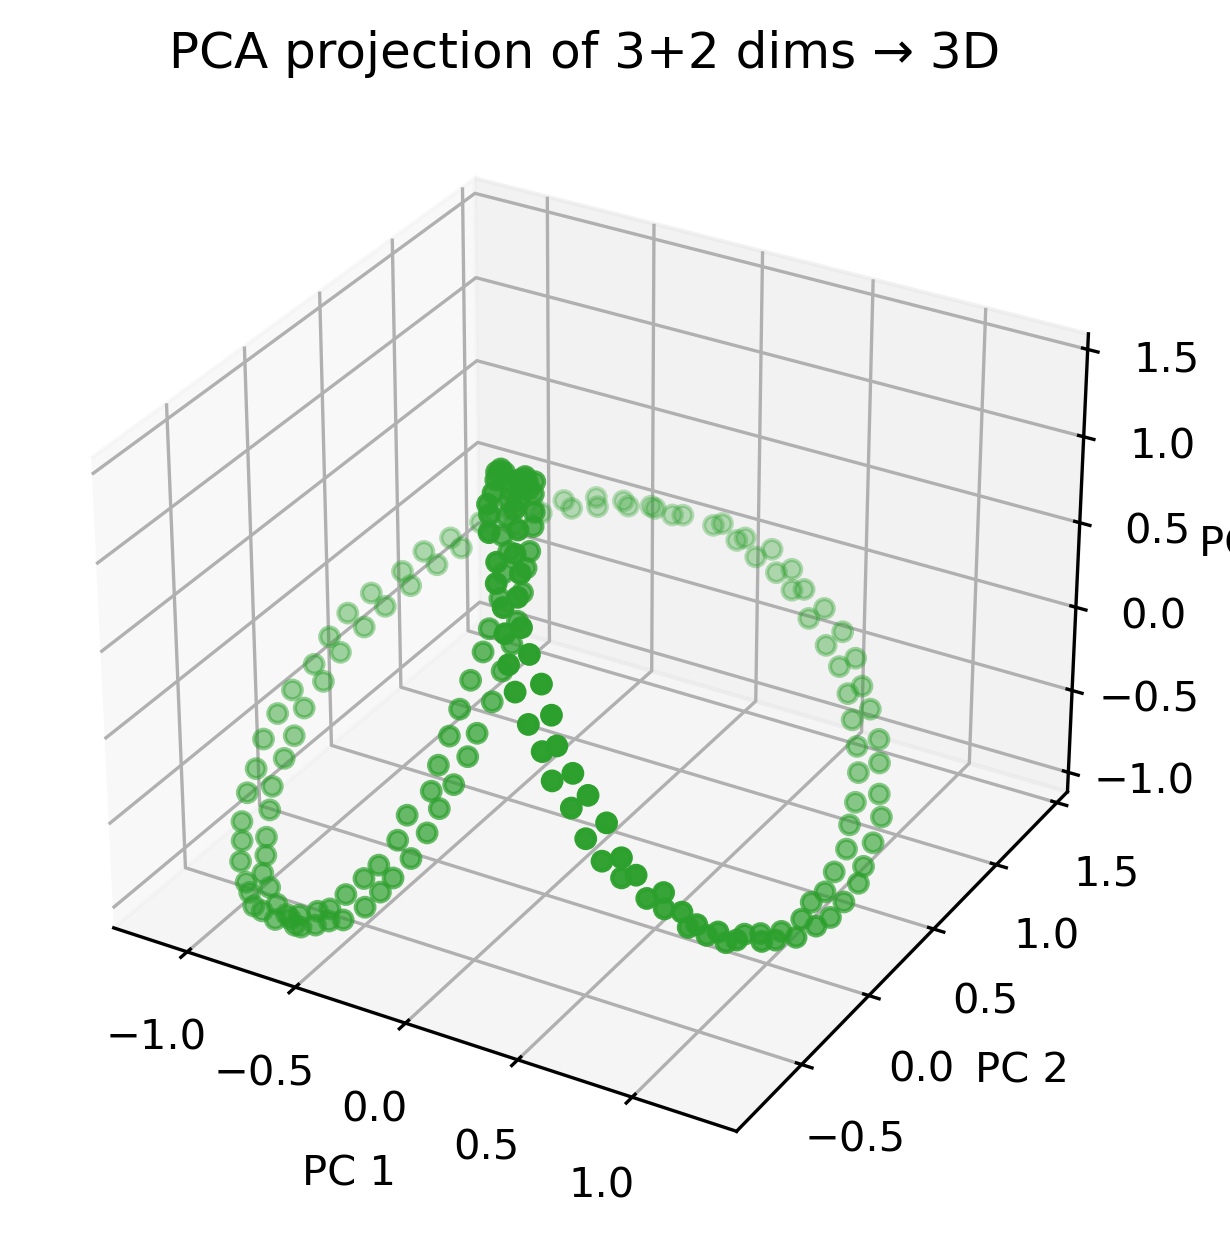
\includegraphics[width=0.75\linewidth]{usage_dataset.png}
    \caption{Projeção PCA do conjunto exploratório com $N=200$ amostras.}
    \label{fig:exploratorio}
\end{figure}

O impacto do grau polinomial aparece na Figura~\ref{fig:exploratorio-sweep}.
O ganho geométrico é evidente ao comparar os graus 1 e~6: o primeiro apenas
captura o esqueleto helicoidal, enquanto o segundo já reproduz os enrolamentos
laterais da trajetória. O gráfico de erro indica retornos rapidamente
decrescentes após o grau~7, quando o RMSE atinge
\num{\explorationOptSevenRmse}. A queda quase linear no painel logarítmico
evidencia que termos de ordem superior refinam as regiões de maior curvatura sem
degradar o condicionamento, efeito habilitado pelas rotinas de regularização
automática discutidas na Seção~\ref{sec:metodologia}.

\begin{figure}[H]
    \centering
    \begin{minipage}{0.48\linewidth}
        \centering
        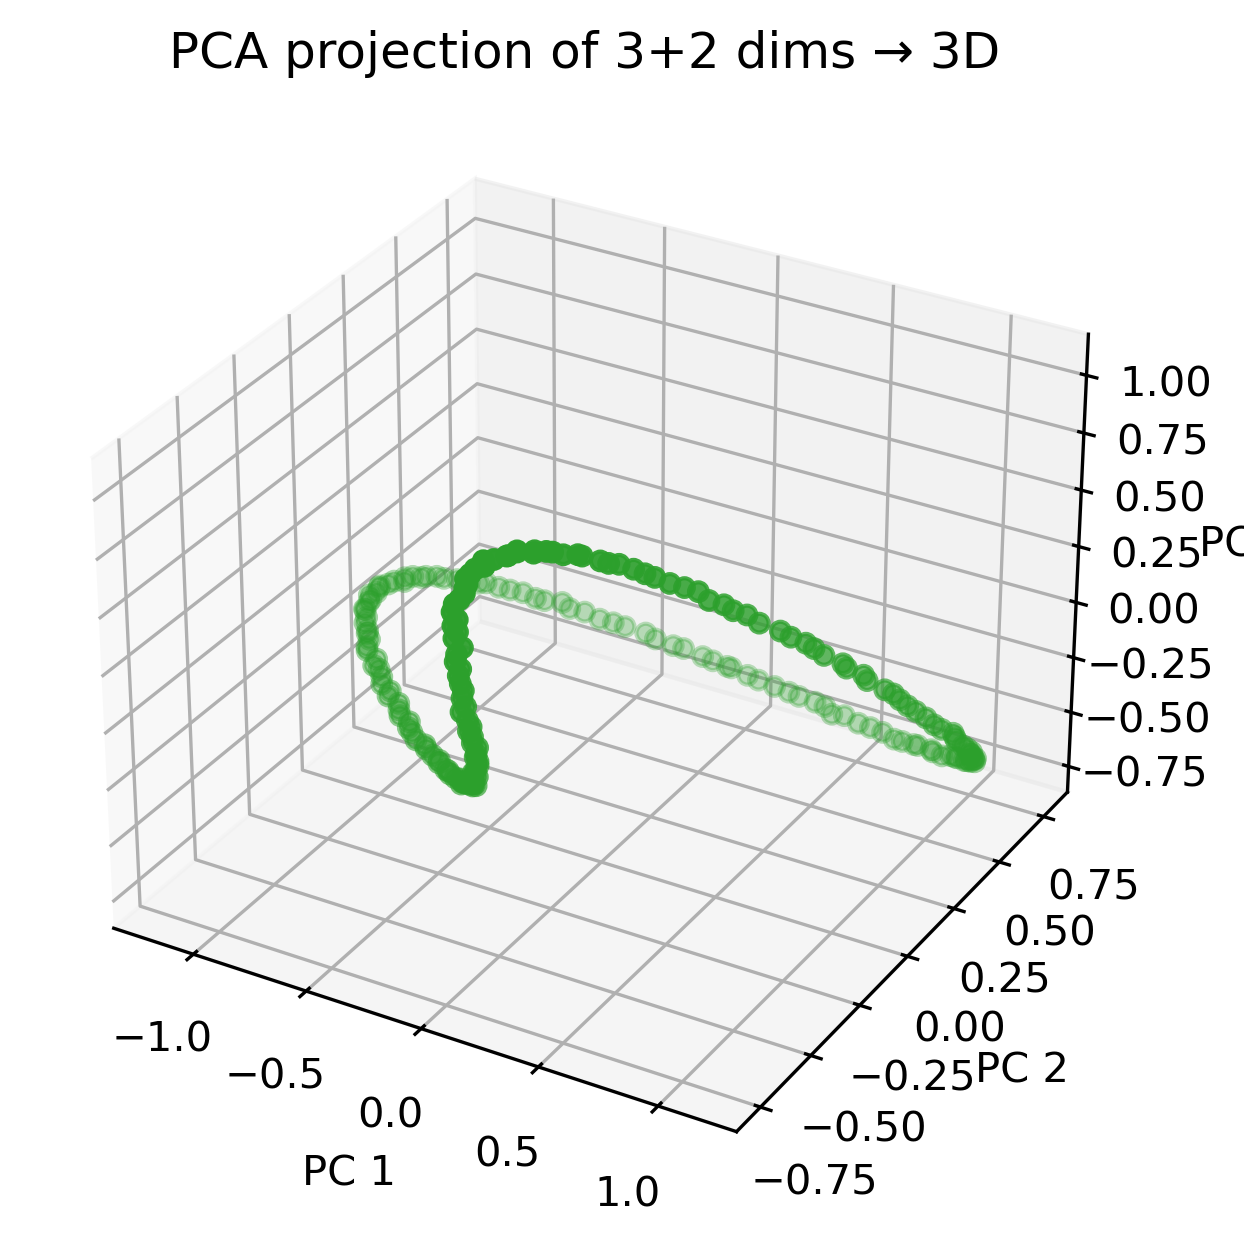
\includegraphics[width=\linewidth]{usage_naive_degree_1.png}\\[0.5em]
        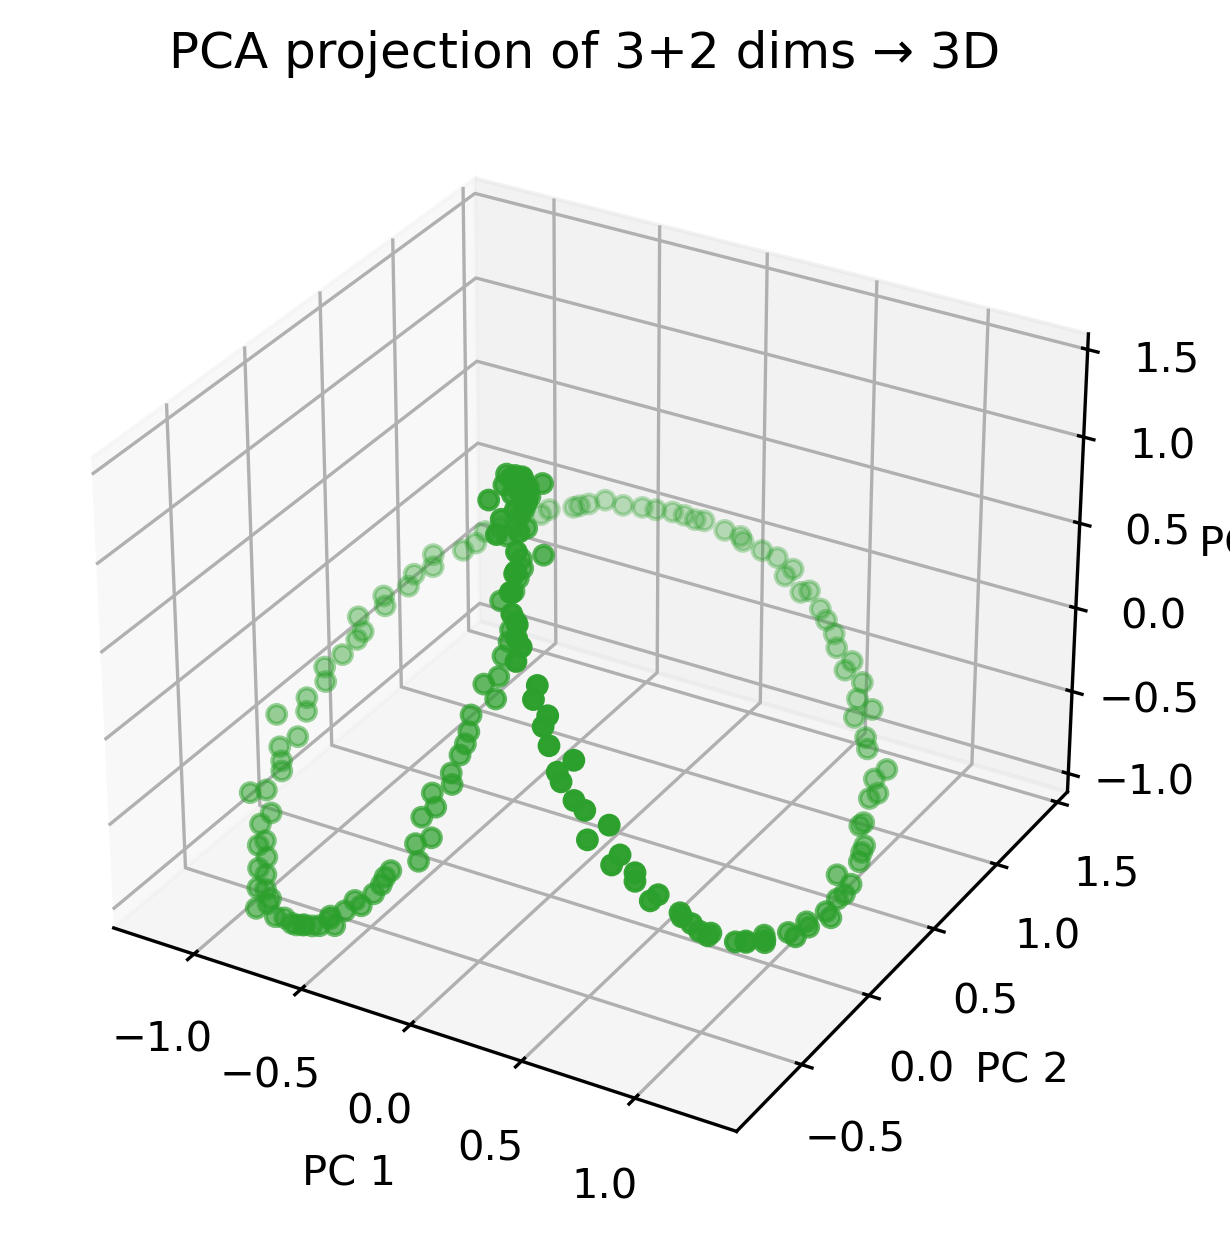
\includegraphics[width=\linewidth]{usage_naive_degree_6.png}
    \end{minipage}\hfill
    \begin{minipage}{0.48\linewidth}
        \centering
        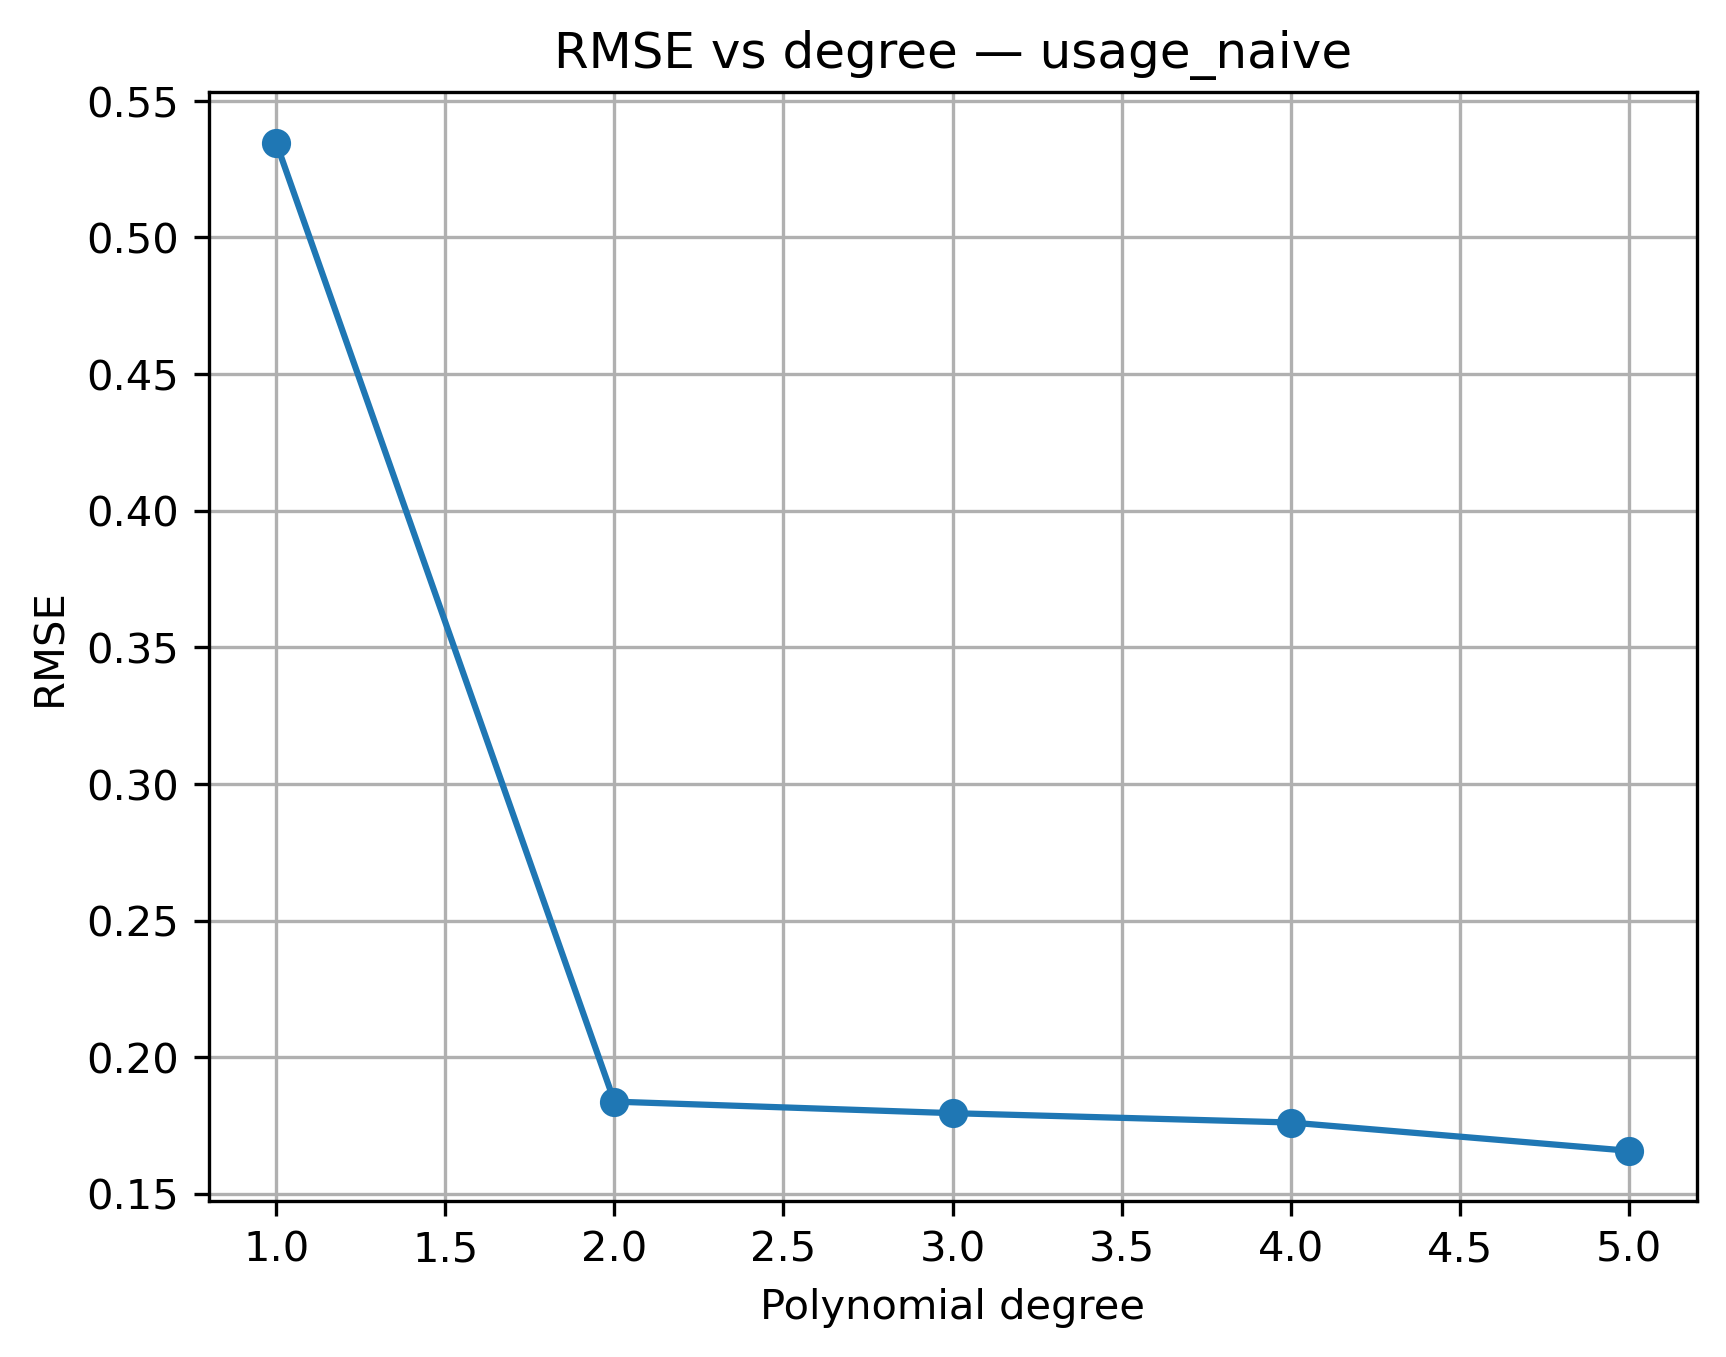
\includegraphics[width=\linewidth]{usage_naive_rmse.png}\\[0.5em]
        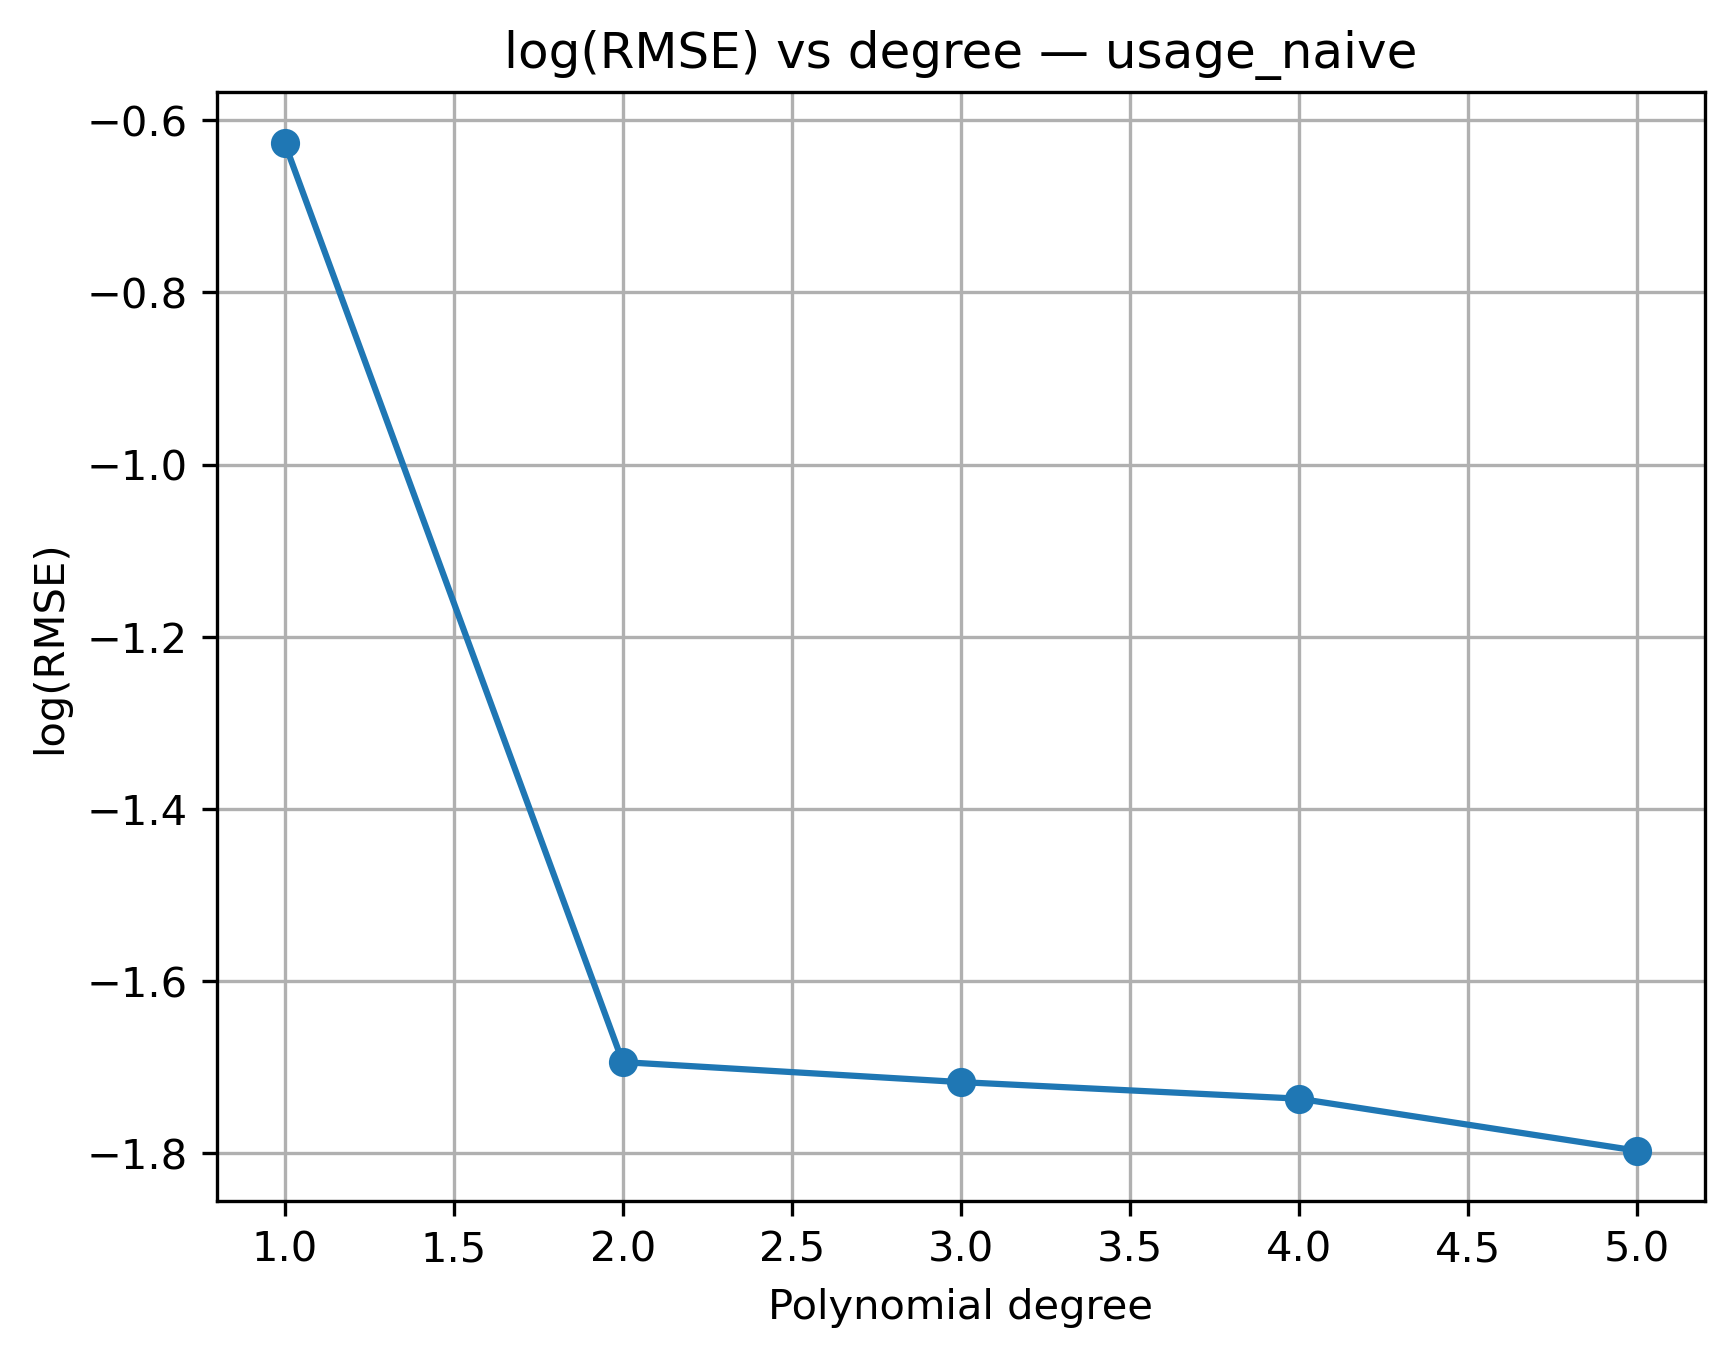
\includegraphics[width=\linewidth]{usage_naive_rmse_log.png}
    \end{minipage}
    \caption{Impacto do grau polinomial. Na esquerda há projeções para os polinômios de grau 1 e 6 e, na direita há o RMSE absoluto e
    logarítmico.}
    \label{fig:exploratorio-sweep}
\end{figure}

\subsection{Problema 2: protótipo 4$\times$4}

O protótipo~4$\times$4 reproduz o conjunto distribuído com o projeto e
combina quatro entradas com quatro saídas correlacionadas. A projeção PCA da
Figura~\ref{fig:target-dataset} mostra que o modelo otimizado acompanha os dois
regimes independentes do problema: as curvas parametrizadas por $t$ e a faixa de
valores controlada por $q$. A trajetória do RMSE cai de
\num{\targetDegreeOneRmse} (grau~1) para
\num{\targetDegreeThreeRmse} (grau~3),
\num{\targetDegreeFiveRmse} (grau~5) e alcança
\num{\targetDegreeSevenRmse} no grau~7, como resume a
Figura~\ref{fig:target-metrics}. O comportamento quase polinomial no painel
logarítmico revela que os termos de grau ímpar absorvem as principais
interações entre os parâmetros, deixando resíduos próximos à precisão numérica.

\begin{figure}[H]
    \centering
    \begin{minipage}{0.48\linewidth}
        \centering
        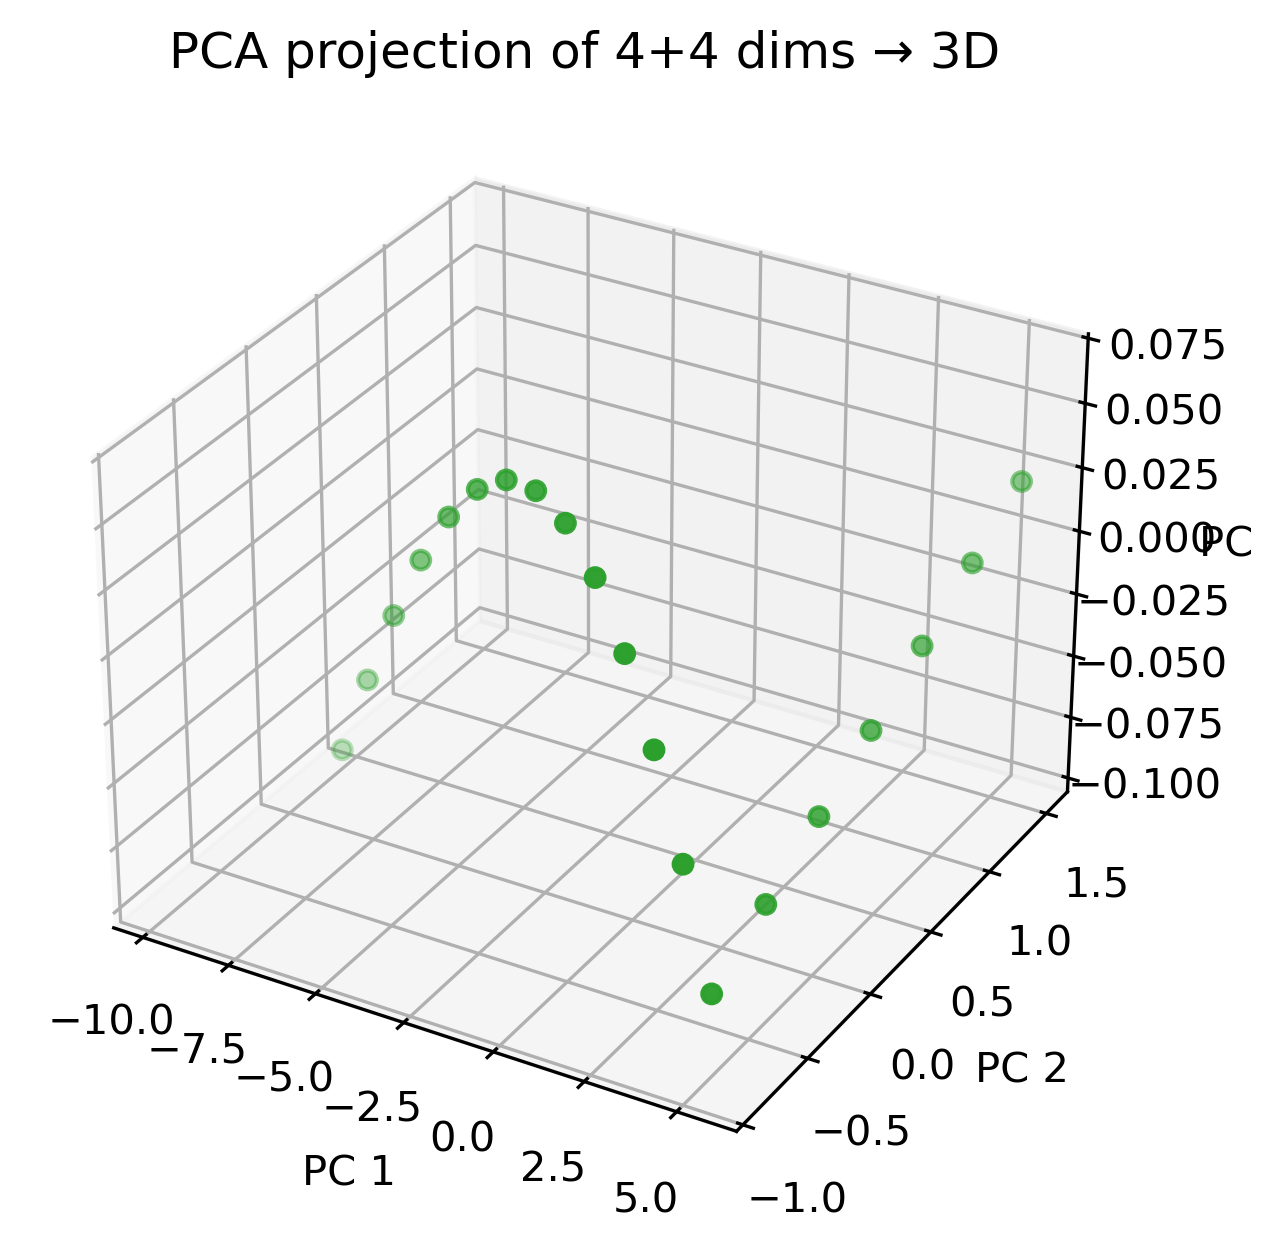
\includegraphics[width=\linewidth]{usage_target_dataset.png}\\[0.5em]
        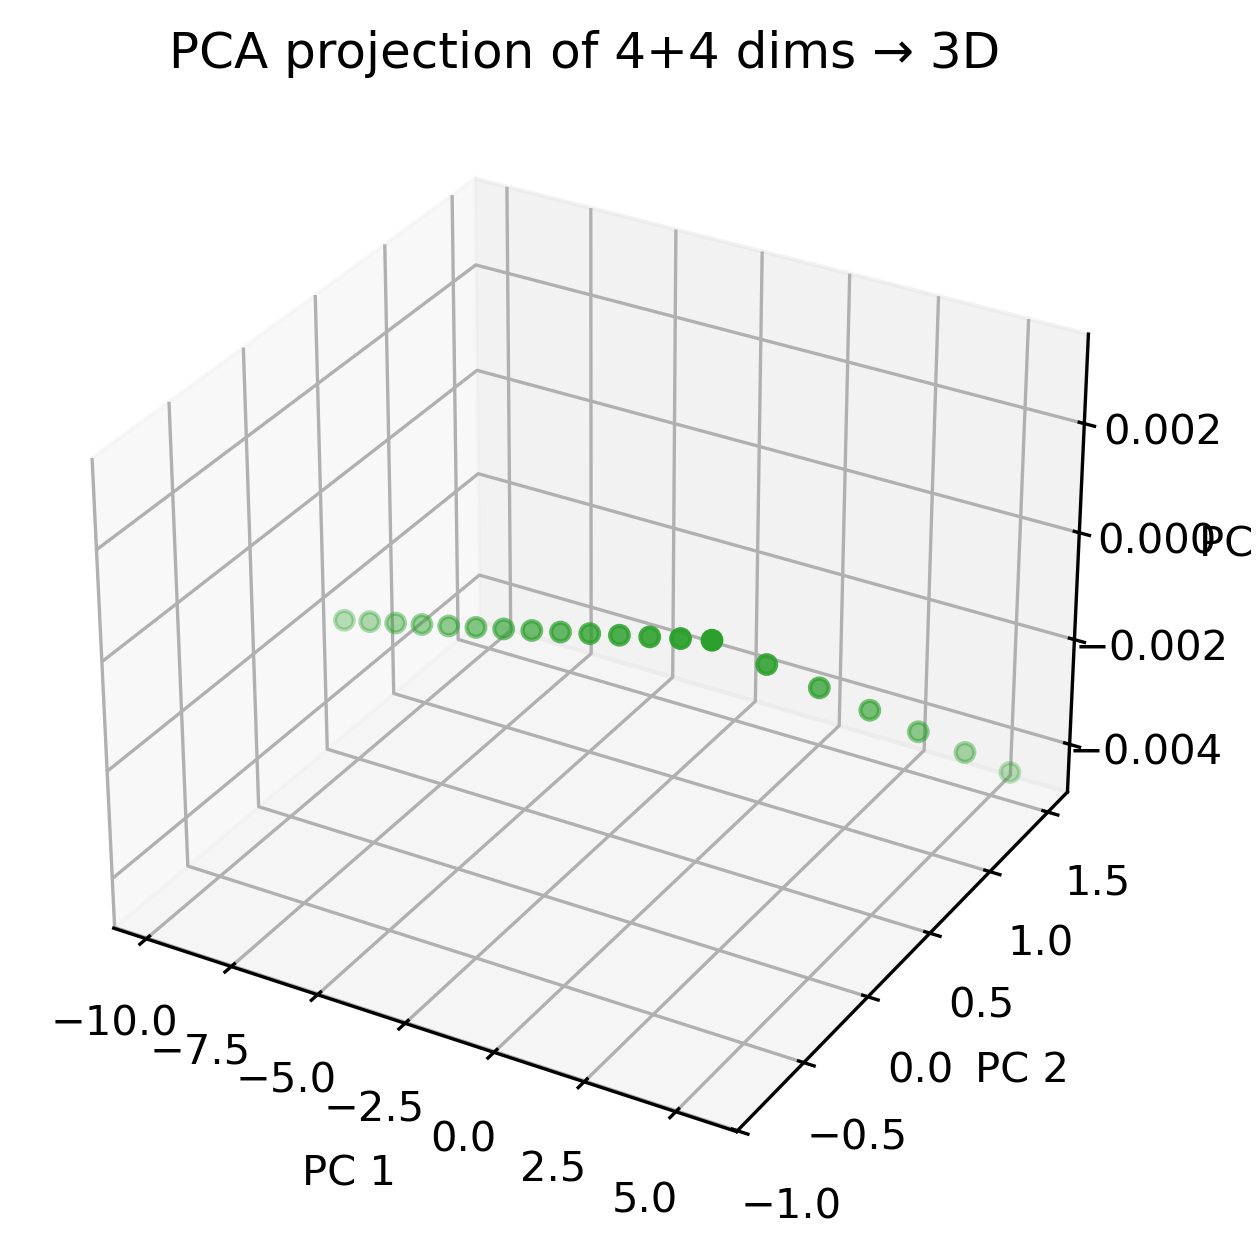
\includegraphics[width=\linewidth]{usage_target_optimized_degree_1.png}
    \end{minipage}\hfill
    \begin{minipage}{0.48\linewidth}
        \centering
        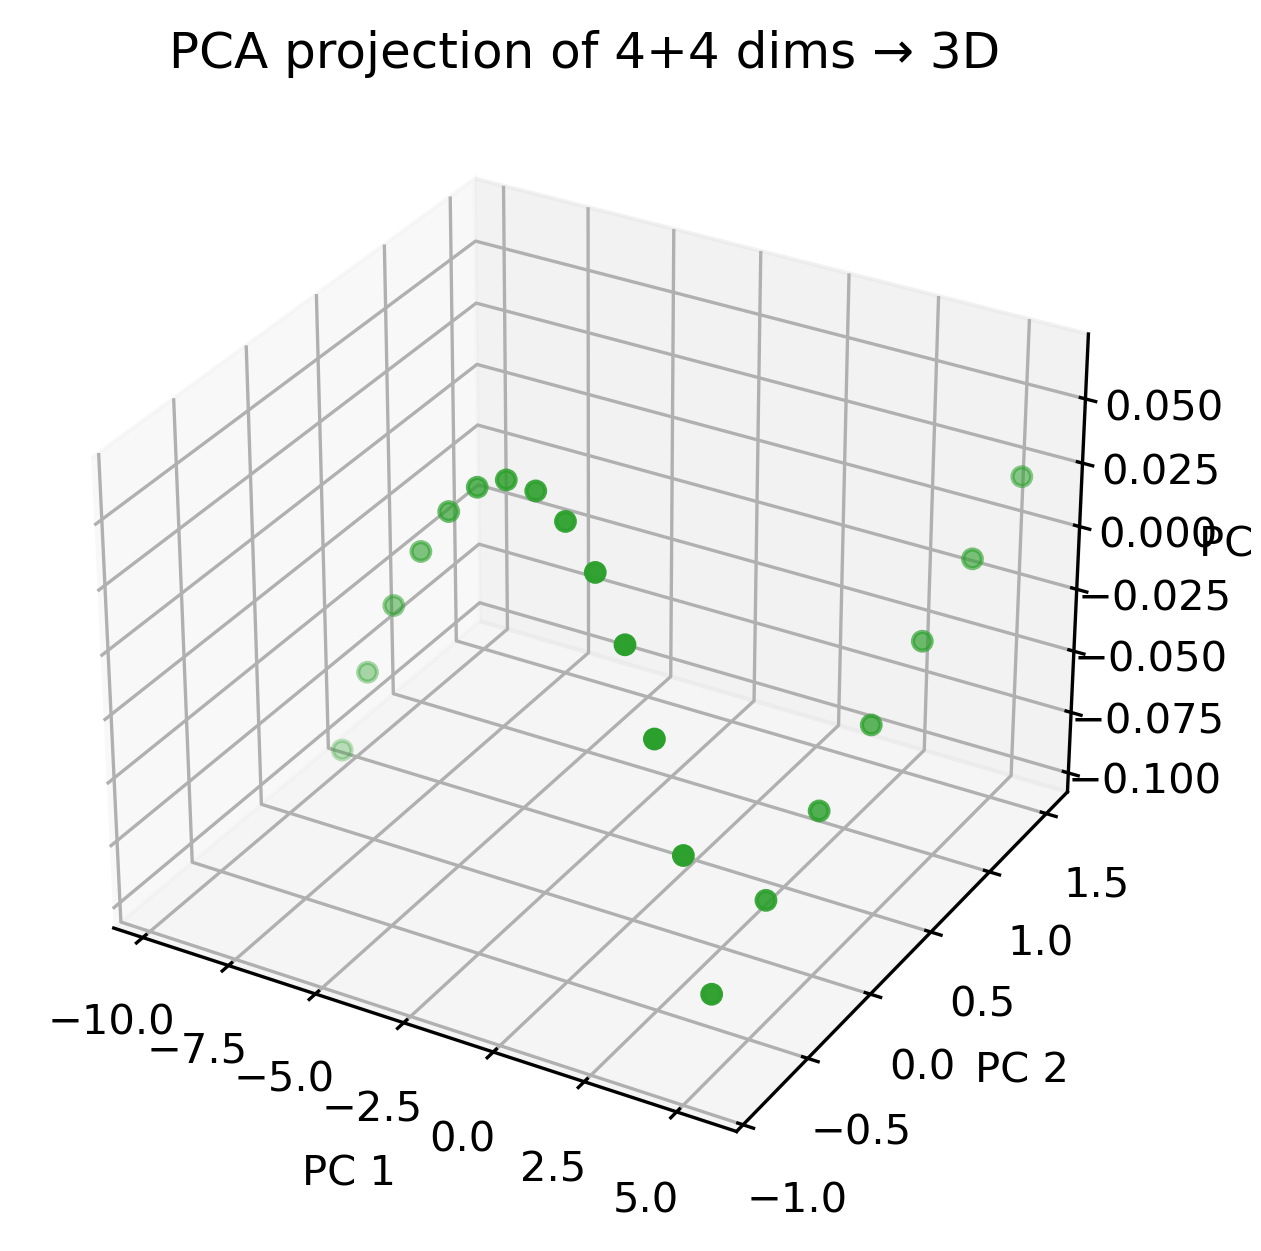
\includegraphics[width=\linewidth]{usage_target_optimized_degree_3.png}\\[0.5em]
        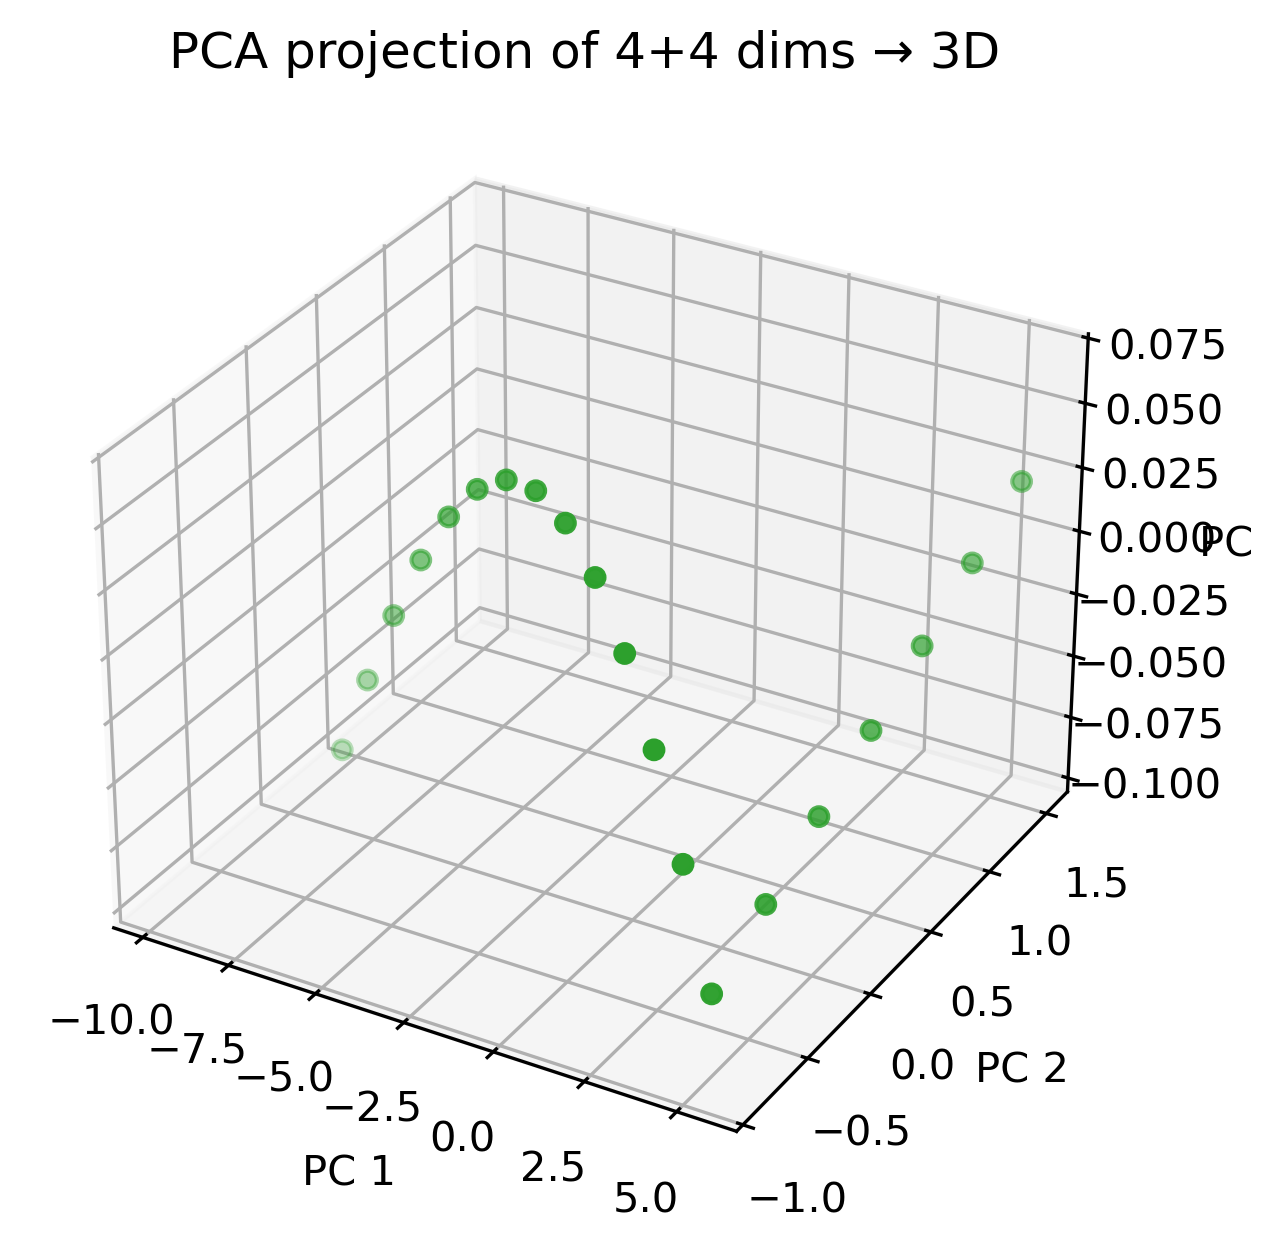
\includegraphics[width=\linewidth]{usage_target_optimized_degree_5.png}
    \end{minipage}
    \caption{Protótipo 4$\times$4: projeção PCA do conjunto (topo esquerdo)
    e reconstruções otimizadas para graus 1, 3 e 5 respectivamente no canto inferior esquerdo, superior direito e inferior direito.}
    \label{fig:target-dataset}
\end{figure}

\begin{figure}[H]
    \centering
    \begin{minipage}{0.48\linewidth}
        \centering
        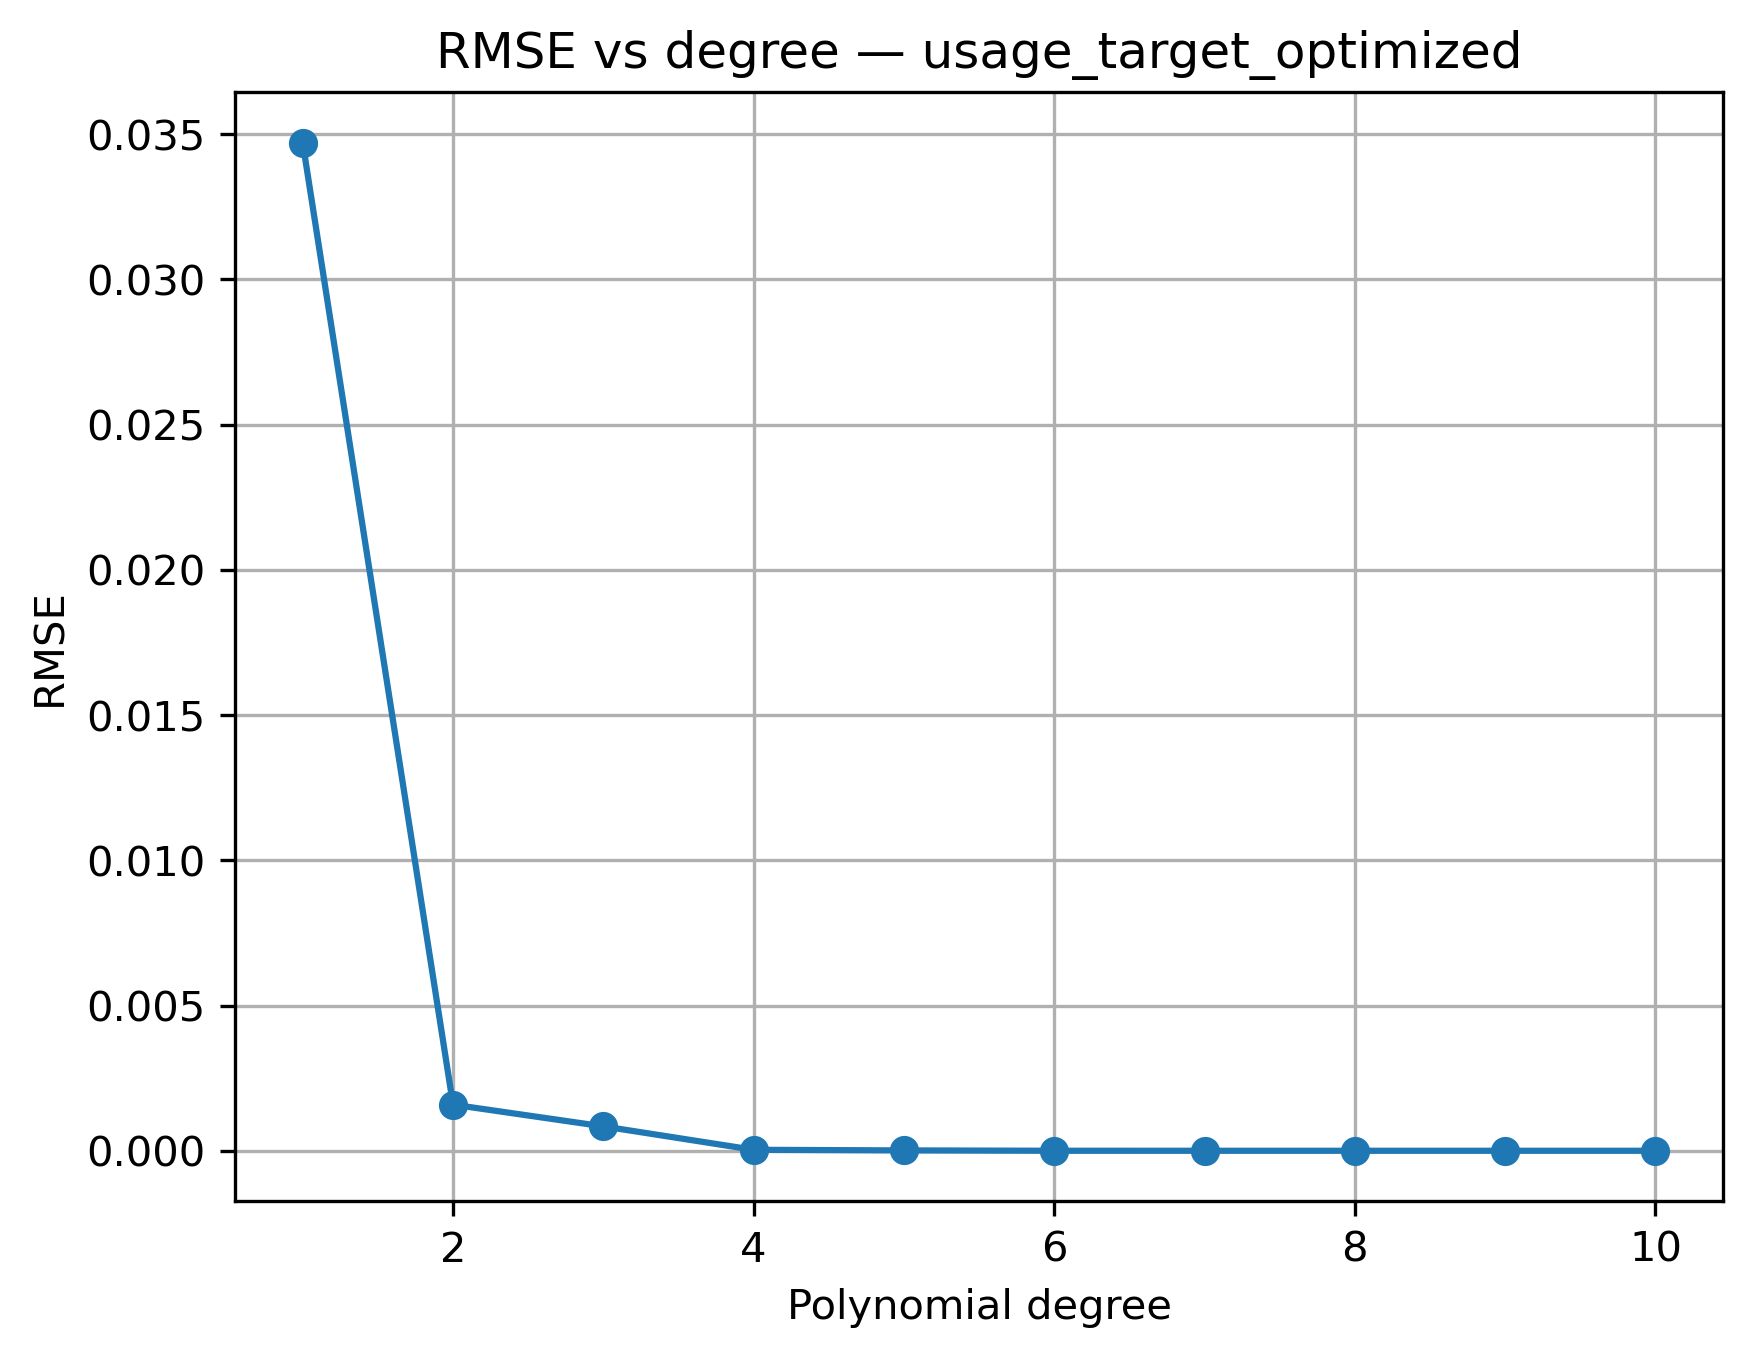
\includegraphics[width=\linewidth]{usage_target_optimized_rmse.png}
    \end{minipage}\hfill
    \begin{minipage}{0.48\linewidth}
        \centering
        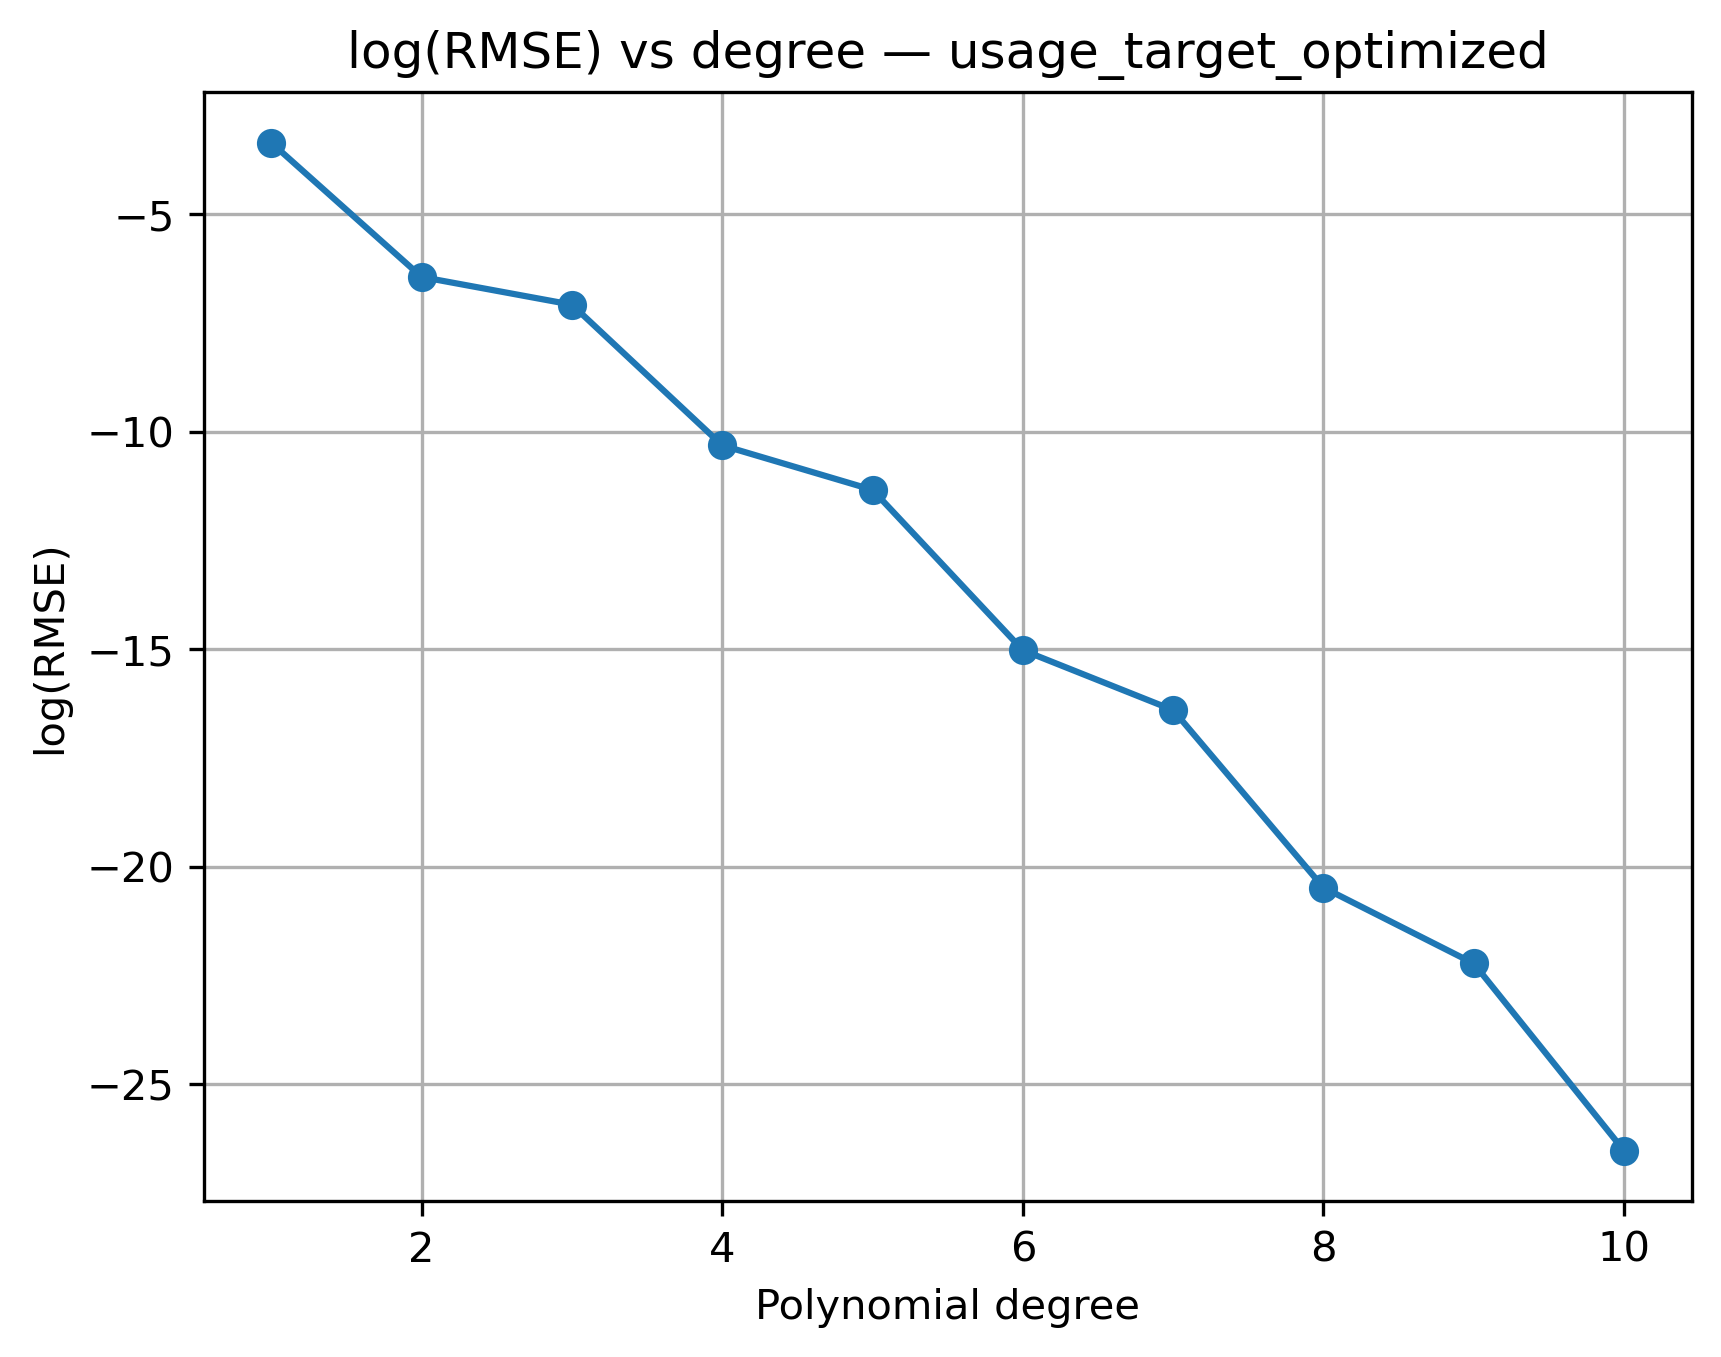
\includegraphics[width=\linewidth]{usage_target_optimized_rmse_log.png}
    \end{minipage}
    \caption{RMSE absoluto e logarítmico para o protótipo 4$\times$4.}
    \label{fig:target-metrics}
\end{figure}

\subsection{Problema extra: superfície da asa}

A superfície ``wing'' aplica nossa técnica em um estudo extra inspirado na aplicação
aeronáutica. A Figura~\ref{fig:wing-dataset} evidencia que o modelo de grau~7 se
ajusta à topologia da asa sem introduzir artefatos, mantendo resíduos entre
$-2{,}26$ e \num{1.98} com média praticamente nula e desvio padrão \num{0.613}.
O sweep de graus da Figura~\ref{fig:wing-metrics} mostra que termos de quarta
ordem já explicam \num[round-mode=places,round-precision=1]{\wingDegreeFourRtwoPercent}\%
da variância, enquanto o grau~7 alcança $R^2 = \num{\wingFullRtwo}$
(\num[round-mode=places,round-precision=1]{\wingFullRtwoPercent}\%) com RMSE de
\num{\wingFullRmse}. A combinação entre projeções PCA e contornos de resíduos
confirma que os erros restantes concentram-se nas bordas da superfície, regiões
com menor densidade de amostras, sugerindo o uso de ponderações futuras para
melhorar a extrapolação.

\begin{figure}[H]
    \centering
    \begin{minipage}{0.48\linewidth}
        \centering
        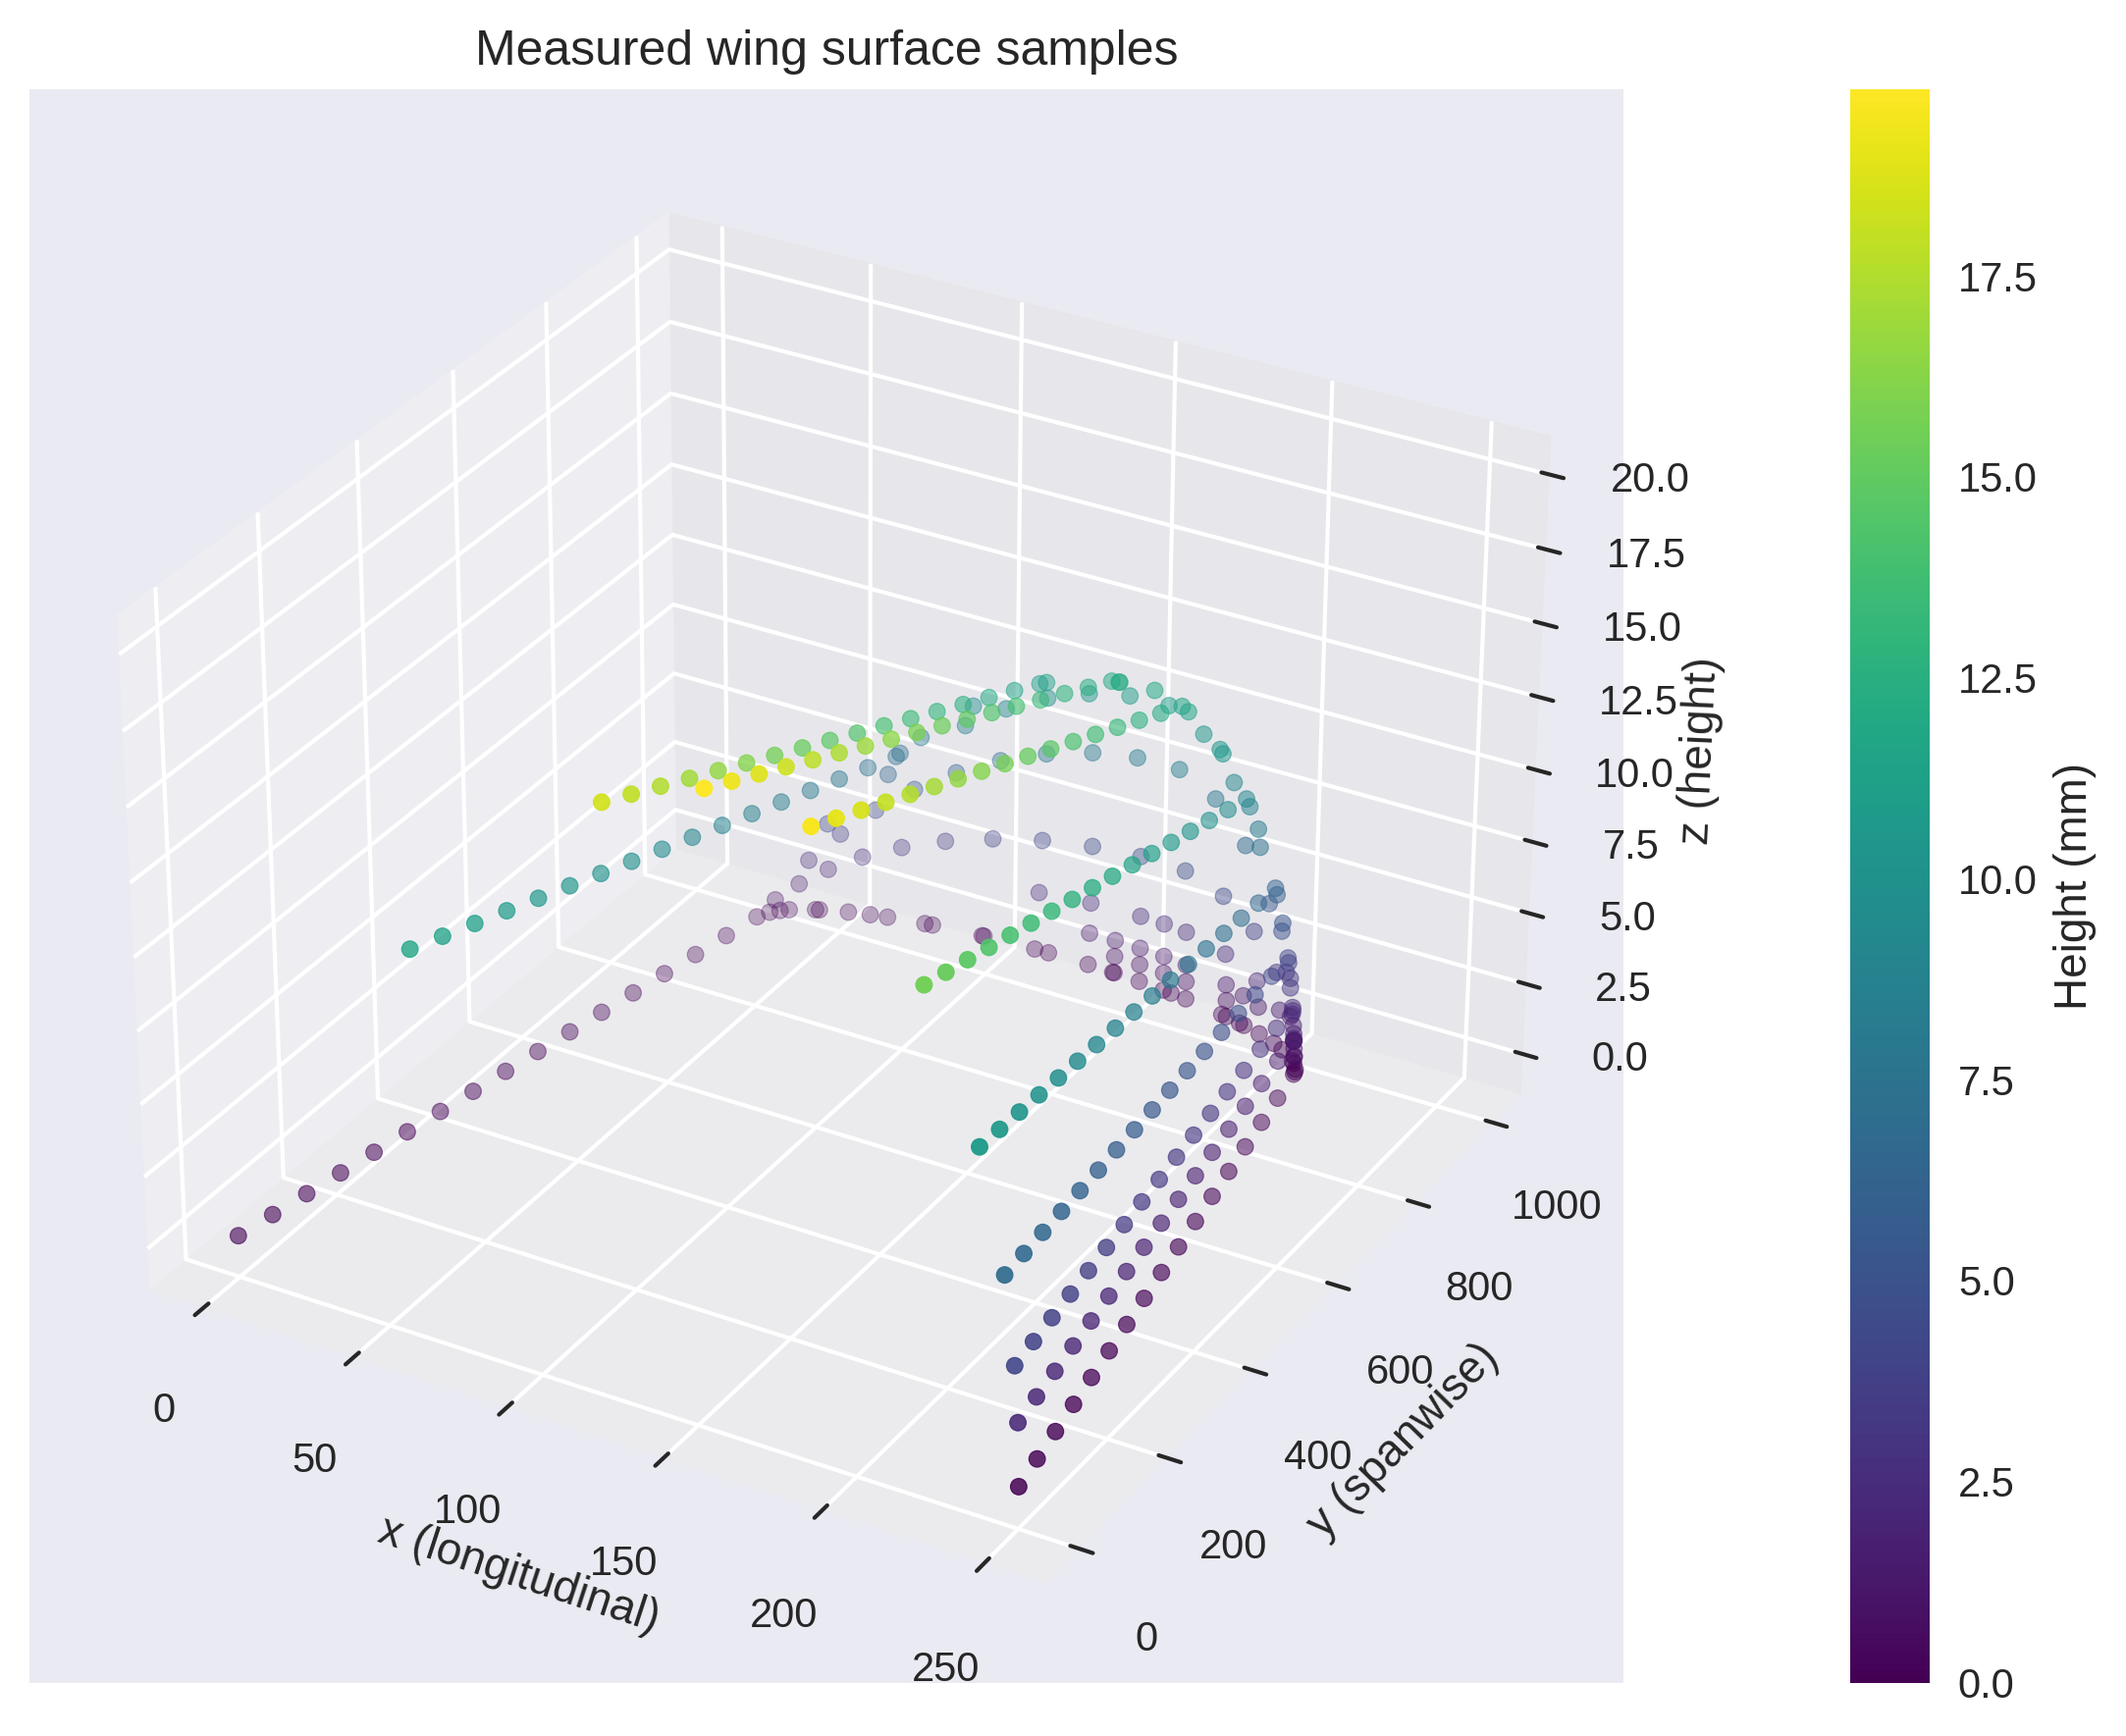
\includegraphics[width=\linewidth]{wing_samples_points.png}\\[0.5em]
        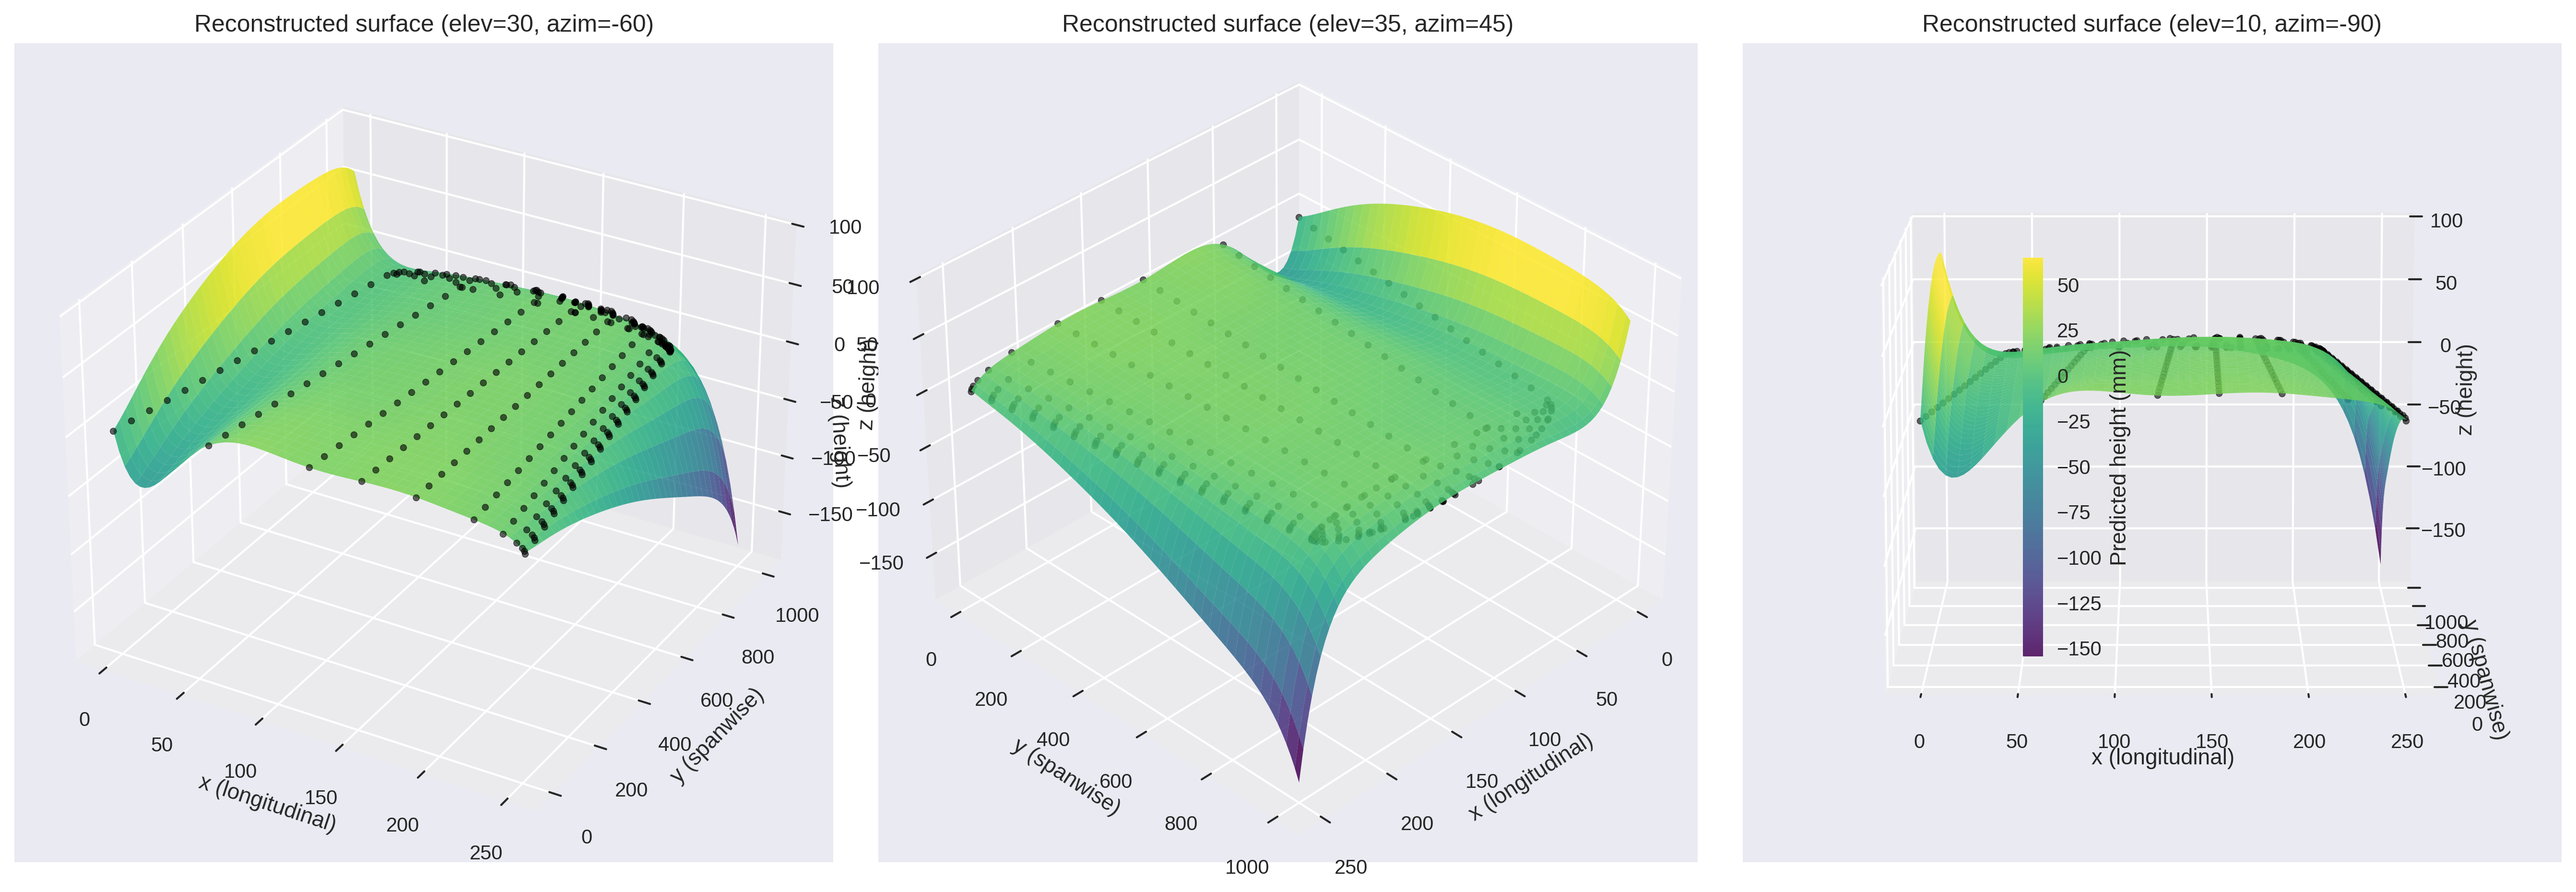
\includegraphics[width=\linewidth]{wing_surface_views.png}
    \end{minipage}\hfill
    \begin{minipage}{0.48\linewidth}
        \centering
        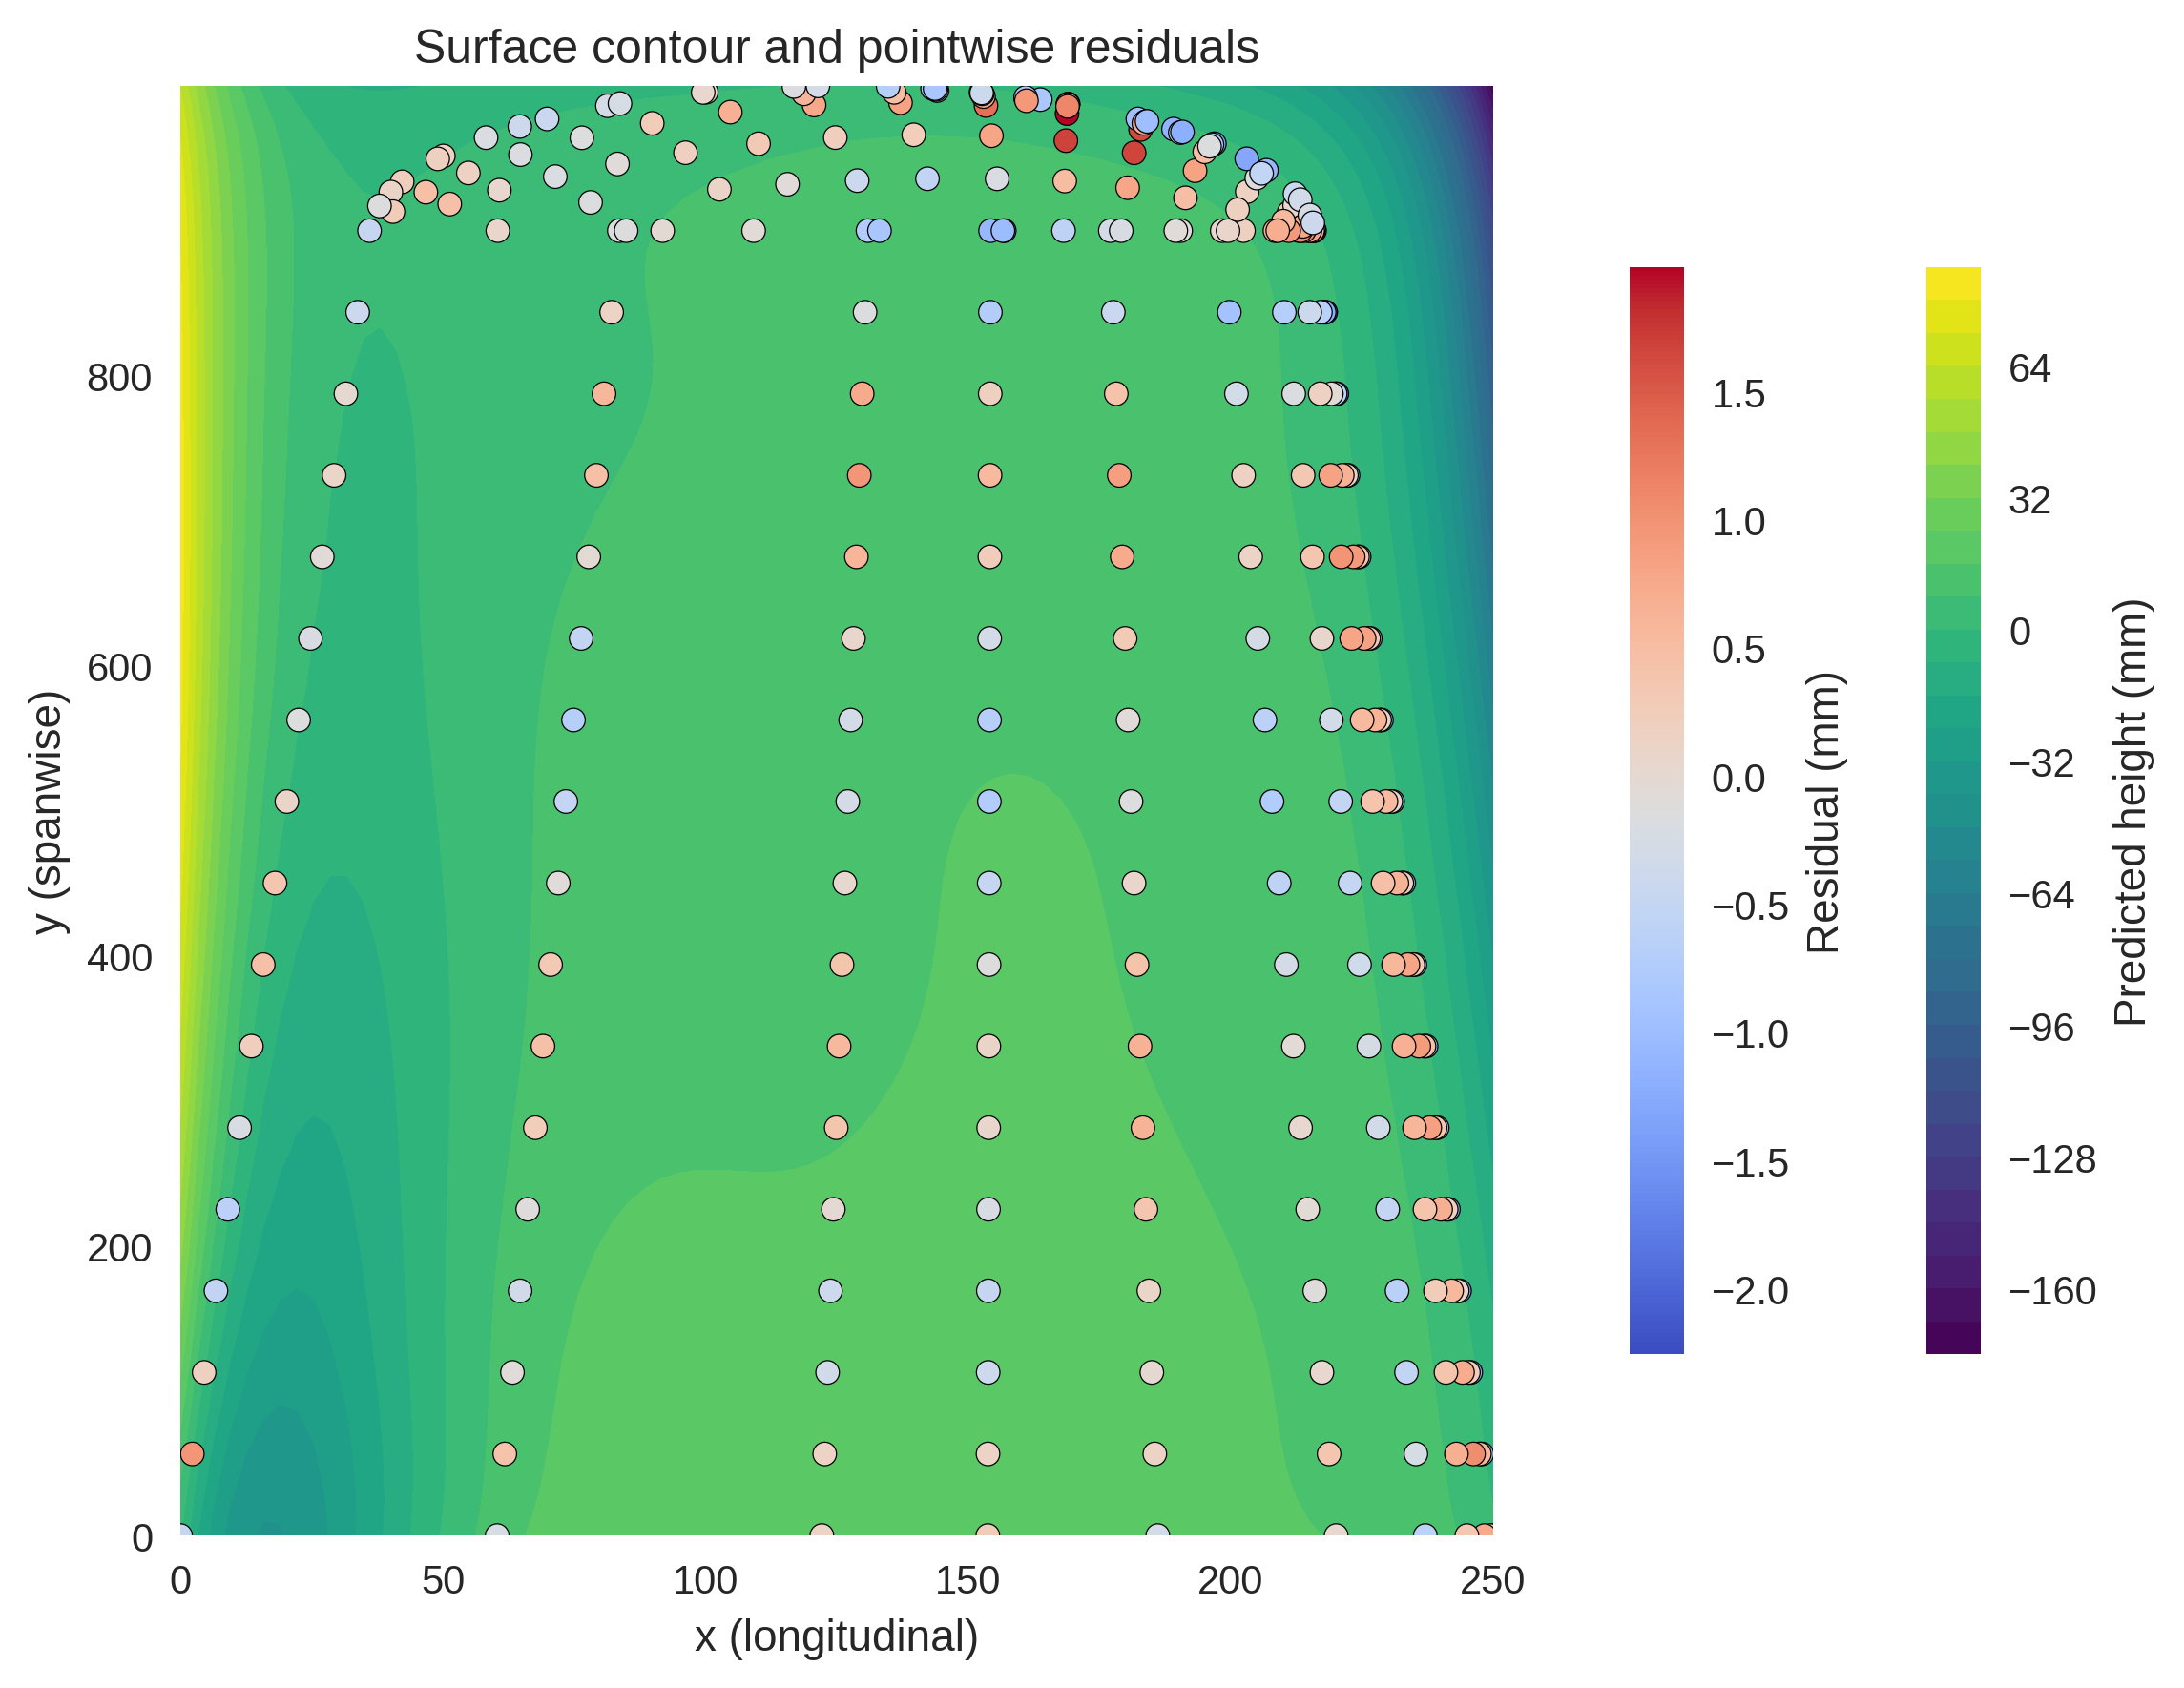
\includegraphics[width=\linewidth]{wing_contour_residuals.png}
    \end{minipage}
    \caption{Conjunto ``wing'': amostras, reconstruções e diagnóstico espacial
    dos resíduos.}
    \label{fig:wing-dataset}
\end{figure}

\begin{figure}[H]
    \centering
    \begin{minipage}{0.48\linewidth}
        \centering
        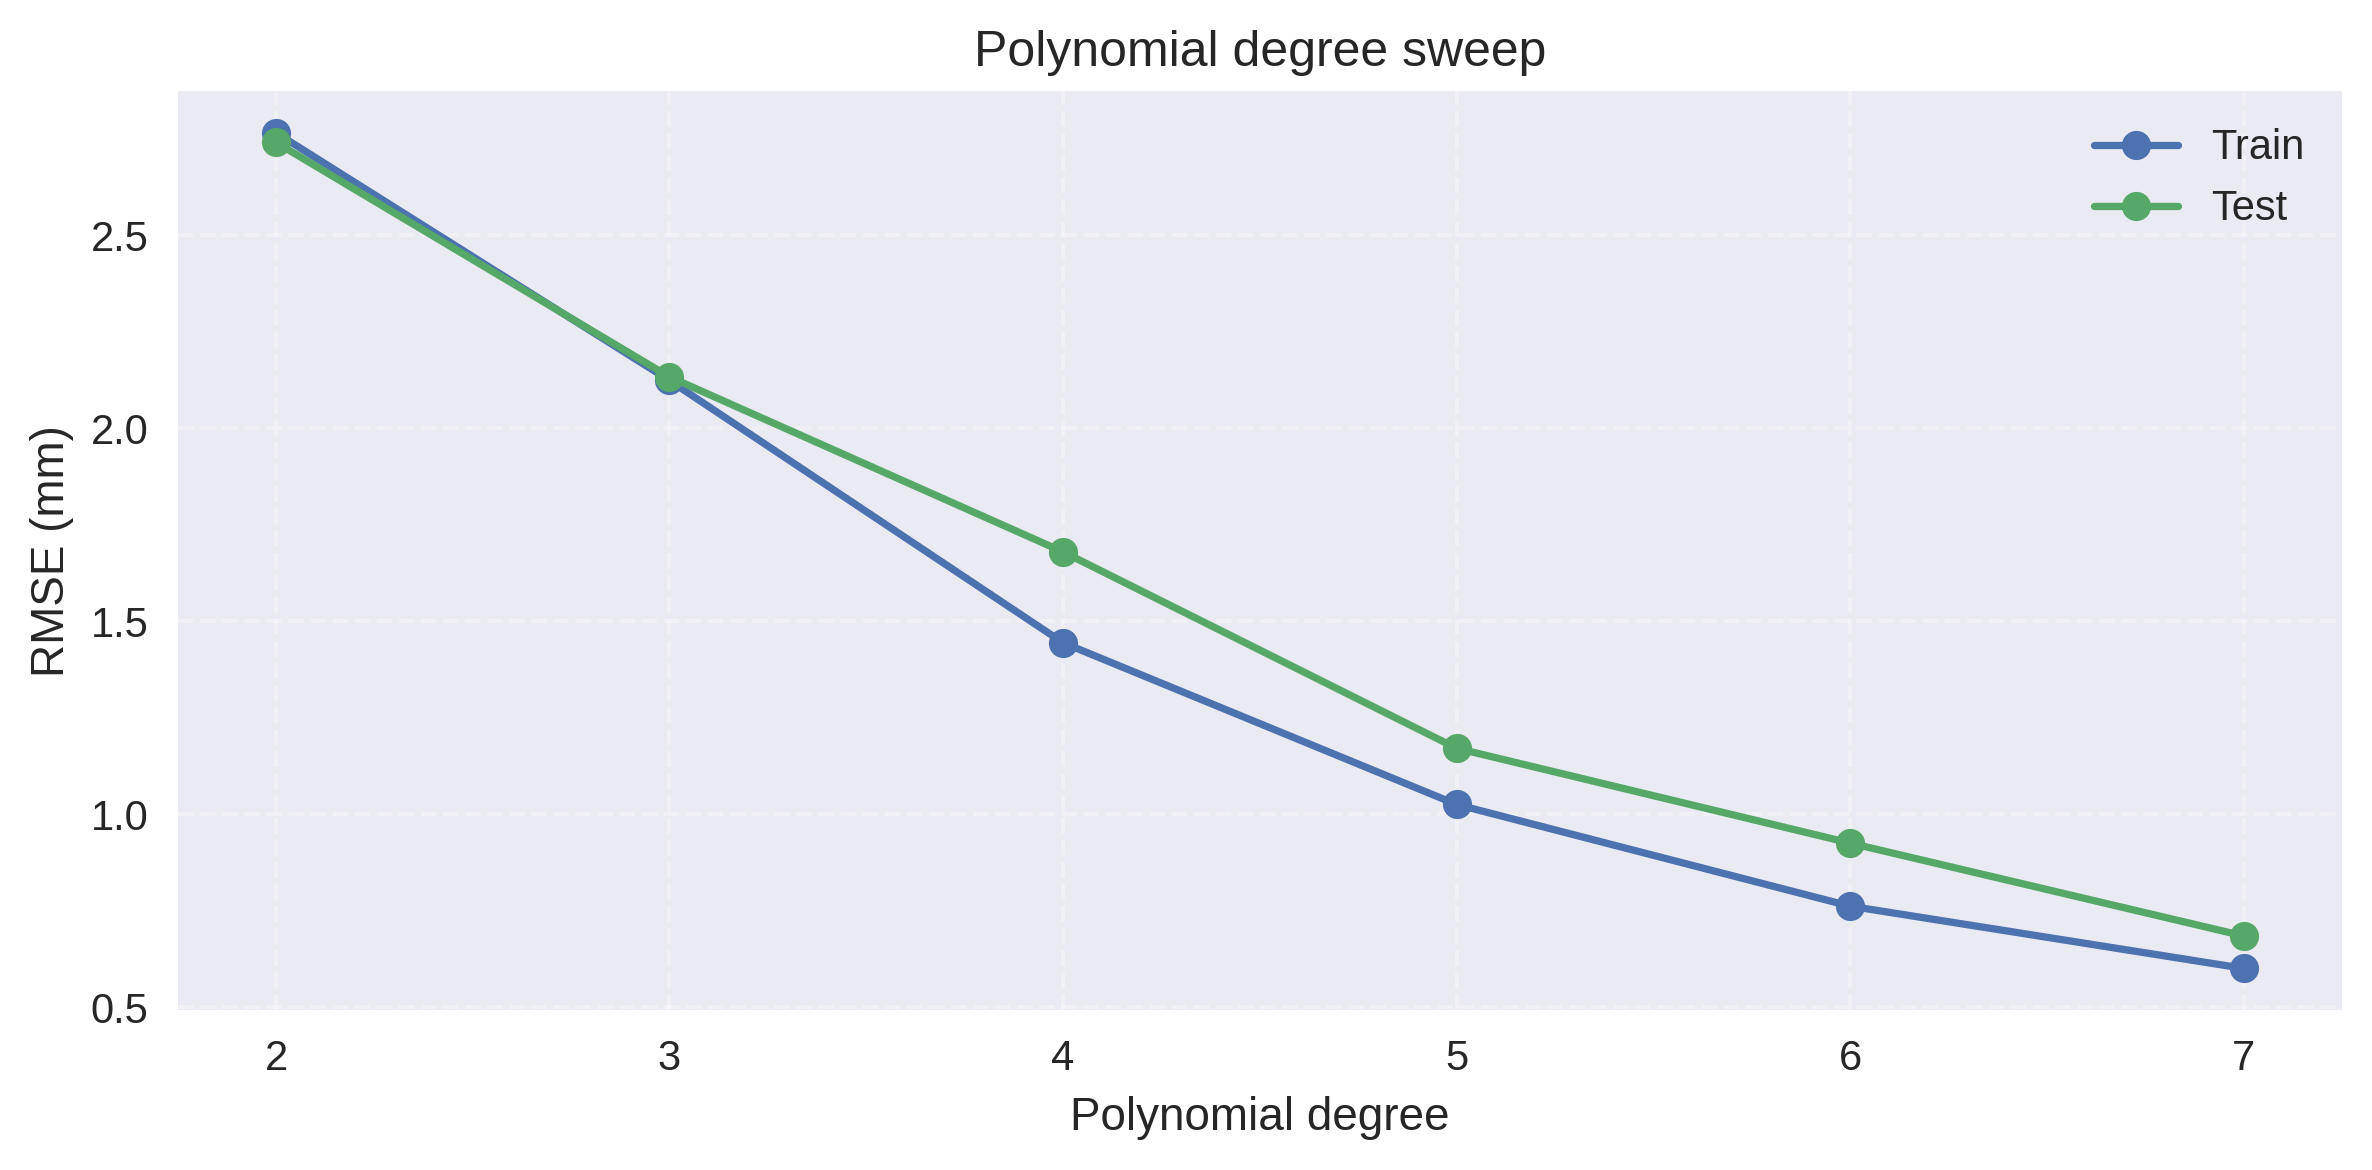
\includegraphics[width=\linewidth]{wing_degree_sweep.png}
    \end{minipage}\hfill
    \begin{minipage}{0.48\linewidth}
        \centering
        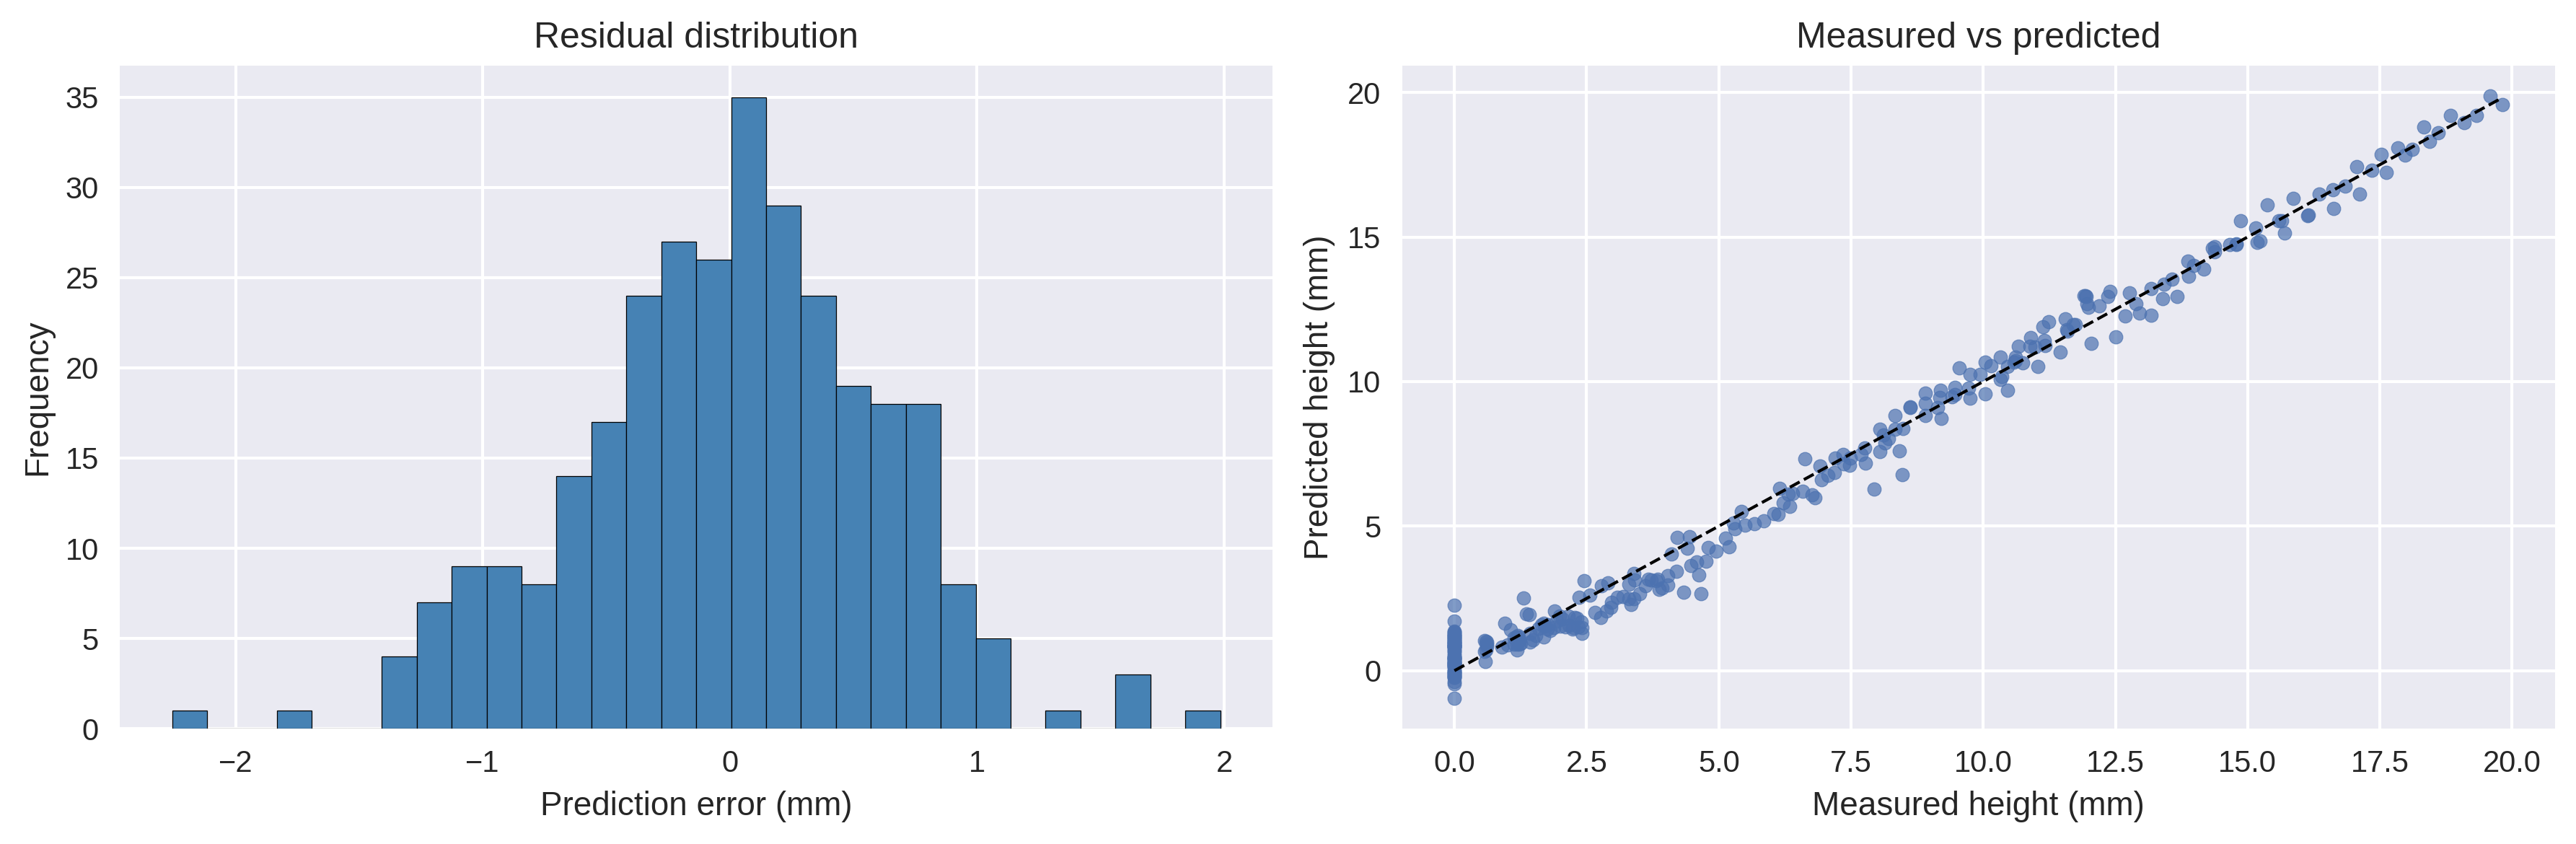
\includegraphics[width=\linewidth]{wing_residual_diagnostics.png}
    \end{minipage}
    \caption{Problema extra ``wing'': variação do erro com o grau (esquerda) e
    distribuição dos resíduos para grau~7 (direita).}
    \label{fig:wing-metrics}
\end{figure}



\subsection{Desempenho computacional}

Os ensaios de desempenho consolidam o impacto das otimizações introduzidas no
\texttt{regkit}. A Tabela~\ref{tab:benchmarks} resume os tempos médios de
execução e o pico de memória coletados para o caso didático com 200 pontos e
polinômios de grau cinco, bem como para o estresse com um milhão de pontos. A
transição da versão simbólica ingênua para o solver vetorizado reduz o tempo em
\num{\benchSpeedup} vezes e limita o uso de memória a apenas
\num[scientific-notation=false,round-mode=places,round-precision=1]{\benchMemPercent}\%
do valor original, sem alterar a acurácia. Já a extensão \textit{out-of-core}
preserva essencialmente o mesmo tempo do solver otimizado nessa escala, 
com custo computacional levemente maior, exibindo
variação relativa de
\num[scientific-notation=false,round-mode=places,round-precision=2]{\benchOocTimeVar}\%
no tempo e
\num[scientific-notation=false,round-mode=places,round-precision=2]{\benchOocMemVar}\%
no consumo de memória.

\begin{table}[H]
    \centering
    \caption{Tempo médio e pico de memória observados nos benchmarks.}
    \label{tab:benchmarks}
    \begin{tabular}{llcc}
        \hline\\
        Cenário & Implementação & Tempo [s] & Memória [MB]\\\\
        \hline\\
        200 pts, grau 5 & Naïve (symbolic) & \num{\benchNaiveTime} & \num{\benchNaiveMem}\\\\
                         & Optimized block solve & \num{\benchOptTime} & \num{\benchOptMem}\\\\
                         & Out-of-core largeP & \num{\benchOocTime} & \num{\benchOocMem}\\\\
        $10^{6}$ pts, grau 5 & Optimized block solve & \num{\benchHighOptTime} & \num{\benchHighOptMem}\\\\
                              & Out-of-core largeP & \num{\benchHighOocTime} & \num{\benchHighOocMem}\\\\
        \hline
    \end{tabular}
\end{table}

O caso de maior carga, ilustrado na Figura~\ref{fig:benchmark_high_load},
demonstra que o fluxo incremental realmente se diferencia quando a memória é o
recurso limitante: ao processar um milhão de pontos, o tempo cai cerca de
\num[scientific-notation=false,round-mode=places,round-precision=1]{\benchHighTimeDrop}\%
e o pico de memória despenca de
\num[scientific-notation=false,round-mode=places,round-precision=0]{\benchHighOptMem}~MB
para
\num[scientific-notation=false,round-mode=places,round-precision=2]{\benchHighOocMem}~MB.
Essa folga viabiliza regressões de alta resolução em estações com recursos
limitados e prepara o terreno para experimentos ainda mais extensos. 

A comparação entre as implementações confirma o objetivo do projeto: 
a versão ingênua serve apenas como referência didática, 
enquanto o solver otimizado é significativamente mais rápido e eficiente, 
sendo indicado para a maioria dos experimentos. 
Já a variante \textit{out-of-core}, 
embora apresente leve aumento no tempo de execução, 
permite o processamento de conjuntos de dados maiores e é recomendada para cenários com restrições de memória.


\begin{figure}[H]
    \centering
    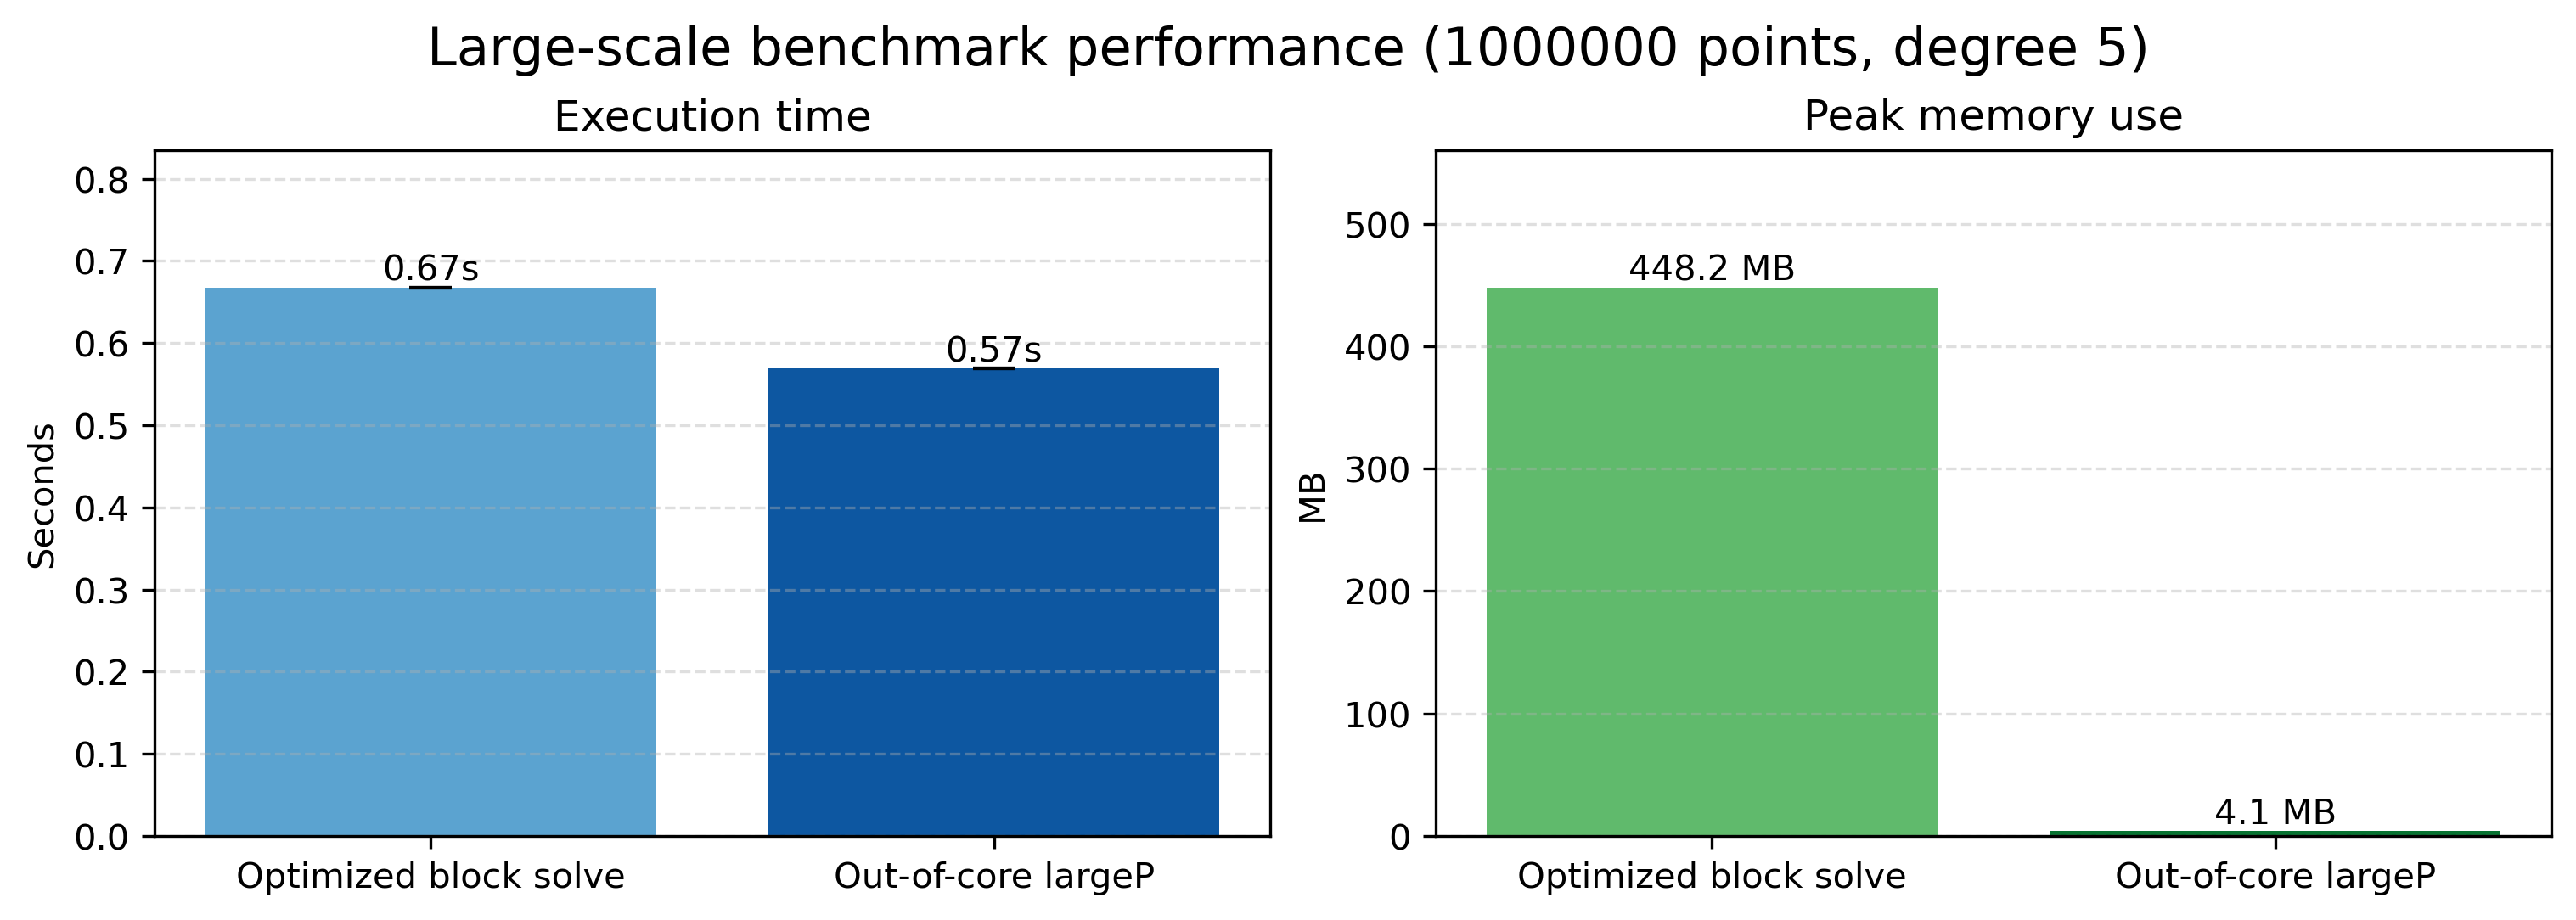
\includegraphics[width=0.9\linewidth]{benchmark_high_load_bars.png}
    \caption{Tempo e memória medidos no estresse com um milhão de pontos.}
    \label{fig:benchmark_high_load}
\end{figure}

\subsection{Condicionamento Numérico}

\pgfplotstableread[col sep=comma]{../../results/ill_conditioned_gram.csv}\illconditioned

\pgfplotstablegetelem{0}{num_points}\of\illconditioned
\edef\illHighPoints{\pgfplotsretval}
\pgfplotstablegetelem{0}{degree}\of\illconditioned
\edef\illHighDegree{\pgfplotsretval}
\pgfplotstablegetelem{0}{cond}\of\illconditioned
\edef\illHighCondRaw{\pgfplotsretval}
\pgfplotstablegetelem{1}{ridge_effective}\of\illconditioned
\edef\illHighRidge{\pgfplotsretval}

\pgfplotstablegetelem{2}{num_points}\of\illconditioned
\edef\illDupPoints{\pgfplotsretval}
\pgfplotstablegetelem{2}{degree}\of\illconditioned
\edef\illDupDegree{\pgfplotsretval}
\pgfplotstablegetelem{2}{cond}\of\illconditioned
\edef\illDupCondRaw{\pgfplotsretval}

\edef\illHighCond{\fpeval{\illHighCondRaw}}

Experimentos controlados confirmaram que certas configurações tornam o bloco de
Gram extremamente mal condicionado.
Um script dedicado\footnote{Disponível no repositório como
\texttt{experiments/run\_ill\_conditioned\_regression.py}, o qual gera a
tabela \texttt{results/ill\_conditioned\_gram.csv}.}
reproduz dois cenários representativos: (i)
\illHighPoints\,amostras equiespaçadas em $[-1,1]$ ajustadas com um polinômio
de grau \illHighDegree, cuja matriz apresenta
$\operatorname{cond}(G) \approx
\num[scientific-notation=true,round-mode=figures,round-precision=3]{\illHighCond}$;
e (ii) \illDupPoints\,amostras coincidentes sob ajuste de grau
\illDupDegree, para as quais $\operatorname{cond}(G)$ é reportado como
\texttt{\illDupCondRaw}, evidenciando a degenerescência da matriz de
Vandermonde.

Denotemos por $V \in \mathbb{R}^{N \times p}$ a matriz de
Vandermonde cujas linhas são os vetores de monômios avaliados em cada ponto
$p_j$ e cujas colunas correspondem às $p=\binom{n+r}{r}$ funções base.
Ao acumular $V^T V$ ao longo das amostras, obtemos precisamente o bloco de
Gram $G$, enquanto a acumulação $V^T \vec{f}$ gera o vetor $\vec{b}$.
Quando as colunas de $V$ ficam quase linearmente dependentes - como ocorre em
graus altos, em domínios muito alongados ou em variáveis fortemente
correlacionadas - essa acumulação herda a perda de significância e culmina em
um $G$ mal condicionado.

Para mitigar tais problemas, o solver \texttt{regression\_optimized} foi projetado para identificar automaticamente situações de mal condicionamento e, nesses casos,
ele substitui a resolução em blocos por uma chamada a
\texttt{numpy.linalg.lstsq}, enquanto \texttt{regression\_largeP} mantém a
decomposição, porém injeta automaticamente uma regularização de magnitude
\num[scientific-notation=true]{\illHighRidge} no sistema, conforme registrado
para ambos os cenários analisados.


\section{Conclusão}

A consolidação computacional confirmou as expectativas teóricas estabelecidas
nas seções iniciais. A implementação simbólica serviu como guia para validar
a correta geração dos termos e possibilitou comparar diretamente os resultados
com as versões otimizadas. O uso de matrizes de projeto vetorizadas e a
decomposição em blocos reduziu o tempo de treinamento em duas ordens de
grandeza, abrindo espaço para experimentos com milhares de amostras e graus
médios. Por fim, os experimentos demonstraram que o ganho de fidelidade com o
aumento de $r$ apresenta retornos decrescentes, reforçando a necessidade de
critérios adaptativos ou regularização adicional em aplicações de maior escala.

Como continuidade direta, pretendemos explorar outros conjuntos de funções base
- como polinômios ortogonais, funções radiais, splines e wavelets - além de
investigar estratégias de seleção automática de grau polinomial e
regularização adaptativa para cenários com ruído não gaussiano. Outro
desdobramento relevante é generalizar a estrutura da regressão para acomodar
funções alvo com características heterogêneas, incluindo dados tensoriais e
categorias discretas. Essas extensões visam ampliar a aplicabilidade do método
em diferentes domínios, como aprendizado de dinâmica de sistemas, modelagem
física e análise de dados multidimensionais.



%\bibliographystyle{alpha}
%\bibliographystyle{unsrt}
\bibliographystyle{ieeetr}
\bibliography{../../paper/common/refs}

\end{document}
